%\documentclass[12pt,article]{memoir}
\documentclass[12pt,a4paper]{article}

%---------------------- MACROS -----------------------
\usepackage{/Users/jesusvillotamiranda/Documents/LaTeX/JVM_Macros}
%----------------------------------------------------

\usepackage{authblk} % to write the title with the authors
\usepackage{booktabs} % when using \documentclass[12pt,a4paper]{article}, you need to load this

%%%%%%%%%%%%%%%%%%%%%%%%%%%%%%%%%%%%%%%%%%%%%%%%%%%%%
%%%%%%%%%%%%%%%%%%%   TITLE     %%%%%%%%%%%%%%%%%%%%%
%%%%%%%%%%%%%%%%%%%%%%%%%%%%%%%%%%%%%%%%%%%%%%%%%%%%%

\title{\textsc{
{\LARGE Network Effects: Using Large Language Models to Map Complex Firm Relationships from News Data}
%\\
%{\large News- }
}}

\author[1]{
{ \bx \bx \bx Insert authors about here
%$^{\dagger}$
%\footnote{
%I am grateful to ...
%I acknowledge financial support from ...
%}
}

%\bx 
%%(\textsc{cemfi})
%{\small
%$\big{<}$
%\noindent $^{\dagger}$CEMFI, Calle Casado del Alisal, 5, 28014 Madrid, Spain 
%$\big{>}$
%
%$\big{<}$
%Email: \href{jesus.villota@cemfi.edu.es}{\texttt{jesus.villota@cemfi.edu.es}}
%$\big{>}$
%}
}

\date{}  % Remove date


%%%%%%%%%%%%%%%%%%%%%%%%%%%%%%%%%%%%%%%%%%%%%%%%%%%%%
\begin{document}
%%%%%%%%%%%%%%%%%%%%%%%%%%%%%%%%%%%%%%%%%%%%%%%%%%%%%
\maketitle
\thispagestyle{empty}  % Suppresses the page number on this page


\begin{abstract}
%----------------------------------------------------
%%\begin{abstract}
%----------------------------------------------------
% 8th October | ~200 words | https://chatgpt.com/share/6704e351-460c-800d-a267-1656528e9ec7
%----------------------------------------------------
In financial markets, news impact stock prices. Despite the postulated \qquote{Efficient Market Hypothesis}, evidence shows inefficiencies, especially with complex information. Research attempting to explain such inefficiencies has often relied on dictionary-based methods, sentiment analysis, topic modeling, and more recently, vector-based models,
%like BERT, 
which still lack a comprehensive understanding of the economic implications of information. Additionally, many studies disregard firm-specific news-implied shocks and overly depend on headlines for analysis. This paper addresses these limitations by leveraging Large Language Models (LLMs) to provide a comprehensive, firm-specific analysis of full news articles. 
%Using a dataset of Spanish business news articles from DowJones Newswires spanning a period of  heightened uncertainty (June 2020 to September 2021), we apply LLMs to understand economic shocks affecting firms, categorizing them by type, magnitude, and direction. The findings illustrate that LLM-based analysis offers superior insights during such volatile periods compared to a benchmark model (KMeans clustering of vector embeddings, which serves as an upper bound for methods lacking comprehensive content analysis). By using LLMs to parse news articles in a way that mimics human processing of the news-implied firm-specific economic shocks, we are able to understand how market reacts to news article, which is evidenced by the out-of-sample profitability of our simple trading strategy.
Using a dataset of Spanish business news from DowJones Newswires during a period of high uncertainty 
%(June 2020 to September 2021), 
we apply LLMs to understand economic shocks affecting firms, categorizing them by type, magnitude, and direction. The findings show that LLM-based analysis provides superior insights during volatile periods compared to a benchmark model (KMeans clustering of vector embeddings). By using LLMs to parse news in a human-like manner, we gain clearer understanding of market reactions to firm-specific information, as evidenced by the profitability of our simple trading strategy.

%----------------------------------------------------
% Previous version | 192 words
%----------------------------------------------------
%In this paper, we explore the incorporation of information in the stock market by building a trading strategy that trades clusters of news. First, we construct the clusters by applying KMeans to the vector embedding representations of the articles. We then propose two algorithms that select \textit{in-sample} the most profitable clusters for trading and project them \textit{out-of-sample} to evaluate the performance of the trading strategy. 
%%\mx 
%In the second part, we perform the clustering by feeding the news articles to a Large Language Model and asking it to classify the type, magnitude, and direction of the shocks implied by each article on the affected firms according to a predefined schema. We then apply the same algorithms for cluster selection as before and check the performance of our trading strategy.
%%
%The results show an inconsistent earnings profile in the test set for the KMeans clustering, while the LLM clustering is able to exploit the information of the articles in a profitable way, creating a consistent earnings profile. These results are robust to hyperparameter variability, such as the number of periods in the holding window and the upper bound on the number of traded clusters. 
%%%%%%%%%%%%%%%%%%%%%%%%%%%%%%%%%%%%%%%%%%%%%%%%%%%%%

%\end{abstract}
%----------------------------------------------------
This paper introduces a novel methodology for constructing and analyzing firm networks using Large Language Models (LLMs) applied to news article data. Unlike traditional approaches that rely on simple co-occurrence patterns, our method leverages LLMs to detect and classify meaningful economic relationships between firms. The framework identifies six distinct types of firm relationships: supplier-customer, competitive, partnership, mergers and acquisitions, legal disputes, and other interactions. We develop a mathematical framework that incorporates both directionality (asymmetric relationships) and reflexivity (self-relationships), resulting in a multi-layered network representation. Each layer corresponds to a specific relationship type, with edges weighted by LLM-derived relationship scores. Our methodology enables dynamic network analysis, tracking how firm relationships evolve over time and respond to external events. This enhanced network representation offers new insights into supply chain structures, competitive landscapes, and the propagation of economic shocks through firm networks.

\bx

\noindent\textbf{JEL Codes:}  C45, C55, G14, L14

\noindent\textbf{Keywords:} Firm Networks, Large Language Models, Natural Language Processing, Network Analysis, Corporate Relationships
\end{abstract}


%%%%%%%% TABLE OF CONTENTS %%%%%%%%%%%
\newpage
\tableofcontents
\thispagestyle{empty}  % Suppresses the page number on this page

\newpage
\setcounter{page}{1}
%%%%%%%%%%%% INTRODUCTION %%%%%%%%%%%%%%%%%%
%\section{Introduction, Literature Review \& Structure}
%----------------------------------------------------
%

%----------------------------------------------------
% 18 June 2024 | Raw text from my own writing
%----------------------------------------------------

\hspace{0.5cm} This paper aims to provide a novel and universal approach to analyzing the impact of business news on stock prices. Our approach is novel in that it is the first time that Large Language Models are employed to \textit{comprehensively} analyze the shocks described in business news articles for return prediction purposes, and it is universal in the sense that it does not rely on access to structured metadata from paid news portals, which, in general, are not widely accessible to the common researcher.

\mx 
Our database consists of a set of Spanish business news articles from DowJones spanning June 2020 to September 2021. Such articles are filtered in a way that allows us to extract the firms directly involved in them. In the first exercise, we convert the wording of the articles from text to high-dimensional vector embeddings by using a transformer model. Such representation captures the general contextual and semantic meaning of the text but is not able to capture the subtle nuances of the shocks described there on the affected firms. 

\mx 
We then cluster our news articles by applying the KMeans algorithm to the associated vector embeddings. This procedure delivers 26 clusters of business news, where each cluster usually pools together articles about a firm or set of firms in the same sector. 

\mx 
For each firm affected by an article, a market model is constructed on some window previous to the day where the article's information got incorporated into the market. Such model is then used to construct a beta-neutral strategy that extracts the abnormal returns of the firm after controlling for the market. 
%\mx 
By obtaining the metrics of this strategy and comparing them across clusters, we can obtain a measure of the profitability of each cluster. We then propose two algorithms that exploit this information to select the optimal clusters.
%to build a trading rule. 

\mx 
Finally, a trading rule is constructed by launching trades on the selected clusters over a specific holding period. By projecting the trading rule onto the test set, we obtain a measure of the profitability of the whole procedure out-of-sample. 

\mx 
The strategy based on KMeans clustering of vector embeddings is not able to generate a consistent earnings profile in the test set, which occurs due to the instability of the clustering method. Namely, the distribution of articles through clusters across data splits shows a very inconsistent pattern, which already hints at the fact that signals generated by the trading rule will not be generalizable out-of-sample.

\mx 
In the second part of the paper, we feed the news articles to a Large Language Model (LLM) and ask it to manually parse them. In particular, we ask the LLM to extract the affected firms and to individually classify the shock implied by the article in each affected firm based on a predefined schema. Such schema consists of a classification of news articles' shocks based on three categories: type (demand, supply, financial, technology, policy), magnitude (minor, major), and direction (positive, negative). We can then cluster the articles based on this classification. 

\mx
In this case, the distribution of articles through clusters is very stable across data splits, which indicates that the trading rule will generate signals that will be generalizable across data splits. Indeed, this is confirmed by the out-of-sample performance of the trading strategy, which shows a consistent earnings profile. These results are robust to hyperparameter variability. In particular, we show that the distribution of Sharpe Ratios in the test set for different choices of holding period length and maximum number of traded clusters is right-skewed and centered at positive values.

%----------------------------------------------------
% 29 April 2024 | Raw text from my own writing
%----------------------------------------------------

%This paper aims to provide a novel and universal approach to analyzing the impact of business news on stock prices. Our approach is novel in that it is the first time that Large Language Models are employed to comprehensively analyze the shocks described in business news articles for return prediction purposes, and it is universal in the sense that it does not rely on access to structured metadata from paid news portals, which, in general, are not widely accessible to the common researcher.


%
%\mx 
%We start with an unstructured corpus of textual data, namely Spanish business news articles, which undergoes preprocessing before being fed into the GPT API. Subsequently, we guide GPT in parsing these news articles and generating structured responses using "function calling", i.e., a predefined set of functions and parameters of our writing to rigorously instruct GPT on how to respond. 
%
%\mx
%Such functions prompt GPT to identify various attributes of the article, including its publication datetime, the type of information provided (new information, historical, analysis/comments, marketing) and its scope (firm-level, industry, global). If the scope of the article is at the firm level, we further ask GPT to list the firms that are directly affected by the events narrated therein. For each identified firm, we request GPT to provide its associated stock market ticker (if publicly traded; otherwise, it returns "NaN"), and further, to classify several aspects regarding how the shock pertains to the firm. Specifically, we prompt GPT to classify the type of shock (e.g., demand, supply, regulatory), the expected duration (short-term, long-term, permanent), the magnitude or relevance (minor, mild, major), and the expected impact on the firm's performance (positive, neutral, negative). Lastly, we obtain GPT's own trading signal by putting it in the shoes of a financial advisor tasked with deciding whether to \textit{Long} or \textit{Short} the stock associated with the firm affected by the news article.
%
%\mx 
%The methodological framework outlined above not only facilitates the identification of pertinent metadata but also generates a structured and comparable array of responses, enabling us to progress the analysis to a supervised stage, which consists of two parts.
%
%\mx 
%In the first part, we examine the predictability of stock returns in response to the shocks delineated in the news articles. To achieve this, we will conduct regressions of the stock returns of affected firms on the dummified shock classifications provided by GPT. This analysis will elucidate the direction and significance of shock predictors for return prediction.
%
%\mx 
%In the second part, we will assess the market timing capabilities of GPT through a market timing test. This involves contrasting GPT's decisions with the decisions that should have been made based on realized returns. In other words, we will juxtapose the stock return predictions of GPT, which inform decisions to long or short the stock, with the actual stock return performance of the respective stock.
%
%\mx 
%Finally, we will construct a set of Long-Short portfolios. One of these portfolios will trade shock signals, determining whether to go long or short based on the shock classifications provided by GPT. Another portfolio will be created using GPT's raw market timing capabilities, disregarding the deeper understanding of the news article implied by the shock analysis and categorization.
%
%\mx 
%All in all, our approach allows us to transition from an unsupervised learning procedure with unstructured data to a supervised learning procedure with structured data that enables us to study the stock return predictability of the shocks described by business news articles.
%
%
%%%%%%%%%%%%%%%%%%%%%%%%%%%%%%%%%%%%%%%%%%%%%%%%%%%%%%%%%%%%%%%%%%%%%%%%%%
%%%%%%%%%%%%%%%%%%%%%%%%%%%%%%%%%%%%%%%%%%%%%%%%%%%%%%%%%%%%%%%%%%%%%%%%%%
%%%%%%%%%%%%%%%%%%%%%%%%%%%%%%%%%%%%%%%%%%%%%%%%%%%%%%%%%%%%%%%%%%%%%%%%%%
%%%%%%%%%%%%%%%%%%%%%%%%%%%%%%%%%%%%%%%%%%%%%%%%%%%%%%%%%%%%%%%%%%%%%%%%%%
%
%%\mx 
%%The methodological framework described above not only facilitates the identification of relevant metadata but also produces a structured and comparable set of responses that allows us to advance the analysis further to a supervised stage,
%
%
%%In the first part, we analyze the stock return predictability of the shocks described in the news articles. For this purpose, we will regress the stock returns of the affected firms on the dummified shock classifications made by GPT. This will allow us to shed light on the direction and significance of shock predictors for return prediction. 
%%
%%For the second part, we will analyze the market timing capabilities of GPT by performing a market timing test. Here we will contrast the decision made by GPT with the decision that should have been taken based on the realized returns. In n other words, we will compare the stock return predictions of GPT (which underlie in the decision made to long or short the stock) and the actual stock return performance of the stock in question. 
%
%%Finally, we will construct a set of Long-Short portfolios. One of such portfolio will trade shock signals; that is, it will decide whether to long/short based on the shock classifications made by GPT. Another portfolio will be constructed using GPT's raw market timing abilities (that is, by simply asking GPT to long or short based on the news and without regard to the deeper understanding on the news article implied by the shock analysis and categorization)
%
%
%%in which we study the stock return predictability of the shock analysis and market timing signals generated by GPT.
%
%%Namely, the output from GPT's response consists of a classification of the shocks implied by the news articles. We launch a set of queries to GPT: we ask it to identify the publication datetime of the article, the type of article (set of possible answers: new information, historical, analysis or comments, marketing) and its scope (firm-level, industry, global). If the scope of the article is at the firm-level, then, we ask GPT to list the firms that are primarily and directly affected by the events narrated in the article. Then, for each firm in that list of firms, we prompt GPT to give us its associated stock market ticker (if the company is publicly traded, otherwise, it spits ``NaN'') and we further ask GPT to classify a set of aspects of how that shock relates to the firm in question. In particular, we ask it about the shock type (demand, supply, regulation,...), the expected duration of that shock (set of possible answers: short-term, long-term, permanent), the magnitude or relevance (set of possible answers: minor, mild, or major), and the direction in which that shock is expected to affect the firm's performance (set of possible answers: positive, neutral negative). Further, we ask GPT to provide a trading signal based on the news article; namely, we put GPT in the shoes of a financial advisor having to decide on whether to Long or Short the stock associated to the affected firm based on the events described in the news article. Once we have obtained a structured answer from GPT we can obtain the metadata of the identified firms to analyze the stock return predictability of the shock analysis and market timing signals generated by GPT.
%%
%
%
%
%%In particular, our approach departs from an unstructured dataset of textual data (a corpus of Spanish news articles) that is preprocessed and fed to GPT. At this stage, we direct GPT on how to parse these news articles and generate a structured response through ``function calling'' (i.e., writing a set of functions and parameters to precisely instruct GPT on to output its completions). This methodology allows us to not only identify the relevant metadata but also to obtain a structured and comparable output that places us in the right place to take the analysis to a supervised stage.
%%---
%%
%%At this stage, a set of functions is defined to instruct GPT on how to parse and analyze the news articles. 
%%
%%At this stage, we task GPT to produce a set of answers according to a function schema that we predefined in advance. 
%%
%%
%%---
%
%%
%%. Different from the previous literature, our procedures don't rely on having access to structured metadata from payable news portals, which are not widely accessible to the common researcher. 
%%
%%In other words, our approach is universal in that it doesn't require metadata from news portals that require subscriptions. 
%%
%%In this sense, we obtain all the information by asking GPT. This is an unsupervised learning approach. 
%%
%%How do we get around this? By delegating the identification of all the relevant metadata to GPT. However, this delegation only works if the right textual preprocessing is performed and the right questions are asked to GPT.  
%%
%%The modus operandi consists of starting from an unsupervised learning approach with unstructured textual data (news articles), which we then preprocess and feed to GPT. 
%%
%%Departing from unstructured news article data, we parse those articles by passing them through the GPT API. 
%%
%%
%%This leads GPT to produce a structured output that can then be employed to analyze the stock return predictability of GPT. 
%%
%
%
%
%%Namely, the output from GPT's response consists of a classification of the shocks implied by the news articles. We launch a set of queries to GPT: we ask it to identify the publication datetime of the article, the type of article (set of possible answers: new information, historical, analysis or comments, marketing) and its scope (firm-level, industry, global). If the scope of the article is at the firm-level, then, we ask GPT to list the firms that are primarily and directly affected by the events narrated in the article. Then, for each firm in that list of firms, we prompt GPT to give us its associated stock market ticker (if the company is publicly traded, otherwise, it spits ``NaN'') and we further ask GPT to classify a set of aspects of how that shock relates to the firm in question. In particular, we ask it about the shock type (demand, supply, regulation,...), the expected duration of that shock (set of possible answers: short-term, long-term, permanent), the magnitude or relevance (set of possible answers: minor, mild, or major), and the direction in which that shock is expected to affect the firm's performance (set of possible answers: positive, neutral negative). Further, we ask GPT to provide a trading signal based on the news article; namely, we put GPT in the shoes of a financial advisor having to decide on whether to Long or Short the stock associated to the affected firm based on the events described in the news article. Once we have obtained a structured answer from GPT we can obtain the metadata of the identified firms to analyze the stock return predictability of the shock analysis and market timing signals generated by GPT.
%
%
%% That is, our approach allows us to transition from an unsupervised learning with unstructured data to a supervised learning procedure with structured data. This latter procedure consists of two parts.
%
%
%%%%%%%%%%%%%%%%%%%%%%%%%%%%%%%%%%%%%%%%%%%%%%%%%%%%%%
%%----------------------------------------------------
%% 29 April 2024 | Parsed using GPT (asked it to simply rephrase my text)
%%----------------------------------------------------
%%%%%%%%%%%%%%%%%%%%%%%%%%%%%%%%%%%%%%%%%%%%%%%%%%%%%%
%
%%This paper endeavors to establish a methodical framework for the analysis of business news articles, aiming to transform unstructured news data into structured insights through the utilization of the GPT API.
%%
%%By instructing GPT through a series of predefined functions, we orchestrate the parsing of news articles to yield structured responses. This approach facilitates the extraction of comparable insights, primarily focusing on classifying the shocks conveyed within the articles. Our methodology involves querying GPT to ascertain key attributes of the articles, including publication datetime, article type (such as new information, historical context, analysis, or commentary), and scope (ranging from firm-level to industry or global perspectives).
%%
%%When the scope pertains to specific firms, we prompt GPT to identify the principal firms directly impacted by the events narrated in the article. Subsequently, for each identified firm, we solicit GPT to classify various aspects of the shock, encompassing its type (such as demand, supply, or regulatory), expected duration (ranging from short-term to long-term or permanent), magnitude or relevance (ranging from minor to major), and anticipated direction of impact on the firm's performance (positive, neutral, or negative). Additionally, we task GPT with generating trading signals based on the news articles, simulating the role of a financial advisor deciding whether to Long or Short the stock associated with the affected firm based on the article's content.
%%
%%The initial phase of our study focuses on analyzing the predictability of stock returns based on these shock classifications. Employing regression analysis, we explore the relationship between stock returns of affected firms and the identified shock predictors, examining both the direction and significance of these predictors.
%%
%%Subsequently, we delve into assessing the market timing capabilities of GPT through a rigorous market timing test. This involves contrasting GPT's decisions regarding stock returns with the ideal decisions that should have been made, thereby evaluating the effectiveness of GPT's predictions in real-world market scenarios.
%%
%%In the final phase, we construct a series of Long-Short portfolios to further explore the practical implications of GPT's insights. One such portfolio will trade based on shock signals, leveraging GPT's shock classifications to inform Long or Short decisions. Another portfolio will utilize GPT's raw market timing abilities, disregarding deeper shock analysis, and solely relying on GPT's instantaneous market predictions derived from news articles.
%
%
%
%%%%%%%%%%%%%%%%%%%%%%%%%%%%%%%%%%%%%%%%%%%%%%%%%%%%%%
%%----------------------------------------------------
%% 29 April 2024 | Parsed using GPT (asked it to do whatever it want with my text)
%%----------------------------------------------------
%%%%%%%%%%%%%%%%%%%%%%%%%%%%%%%%%%%%%%%%%%%%%%%%%%%%%%
%%
%%This paper presents a systematic framework for analyzing business news articles using the GPT API. Departing from unstructured data, we employ a structured approach by instructing GPT through predefined functions, enabling the extraction of comparable and analyzable responses.
%%
%%Our methodology begins by parsing articles through the GPT API, directing it to identify key attributes such as publication datetime, article type, and scope. For articles focused on individual firms, GPT identifies the primary affected firms and classifies aspects of the associated shock, including type, duration, magnitude, and expected impact direction.
%%
%%Furthermore, we task GPT with providing trading signals based on the news content, simulating the decision-making process of a financial advisor. This approach lays the foundation for our subsequent analyses.
%%
%%In the first part of the paper, we investigate the predictability of stock returns based on GPT's shock classifications. Through regression analysis, we examine the significance and directionality of these predictors.
%%
%%Subsequently, we assess GPT's market timing capabilities by comparing its stock return predictions with actual performance. This market timing test evaluates the efficacy of GPT's decision-making process in real-world scenarios.
%%
%%Finally, we construct Long-Short portfolios to further explore GPT's capabilities. One portfolio trades based on GPT's shock signals, while another relies solely on GPT's raw market timing abilities, providing insights into the impact of deeper news analysis.
%%
%%By employing this structured approach, we aim to enhance our understanding of the relationship between business news content and stock market movements, leveraging the capabilities of advanced language models like GPT. 
%%
%%
%%
%%

%----------------------------------------------------
%----------------------------------------------------
%%%%%%%%%%%%%%%%%%%%%%%%%%%%%%%%%%%%%%%%%%%%%%%%%%%%%%
%%%%%%%%%%% INTRODUCING THE LITERATURE %%%%%%%%%%%%%%
%%%%%%%%%%%%%%%%%%%%%%%%%%%%%%%%%%%%%%%%%%%%%%%%%%%%%

The foundation of textual analysis in finance, particularly in the predictive analysis of stock returns using economic news, is built upon several key studies that have shaped the current understanding and methodologies employed in this field. These seminal works not only introduced innovative approaches to analyzing textual data but also laid the groundwork for subsequent research that leverages advanced computational techniques.
%%%%%%%%%%%%%%%%%%%%%%%%%%%%%%%%%%%%%%%%%%%%%%%%%%%%%
%%%%%%%%%%%%%%%%%%%%%%%%%%%%%%%%%%%%%%%%%%%%%%%%%%%%%
%%%%%%%%%%%%%%%%%%%%%%%%%%%%%%%%%%%%%%%%%%%%%%%%%%%%%

\mx
\cite{tetlock2007giving}
's study is a pivotal contribution to textual analysis in finance. He examines the predictive power of negative words in a popular column from The Wall Street Journal on subsequent stock returns. His findings indicate that high levels of media pessimism predict lower future returns, suggesting that media sentiment embedded in news content can significantly influence market prices. This research underscores the role of media tone and sentiment in shaping investor behavior and market trends.

\mx
\cite{fang2009media}
explore the impact of media coverage on the stock returns of publicly traded firms. They find that stocks with less media coverage generate higher future returns compared to those with more extensive coverage. This effect is attributed to the media's role in disseminating information to the public, which influences investor awareness and risk perceptions. Their study provides crucial insights into how variations in media attention can affect market dynamics and investor behavior.

\mx
\cite{bollen2011twitter} 
extend the domain of textual analysis into the realm of social media, demonstrating how sentiment derived from Twitter feeds can forecast stock market movements. They analyze the correlation between collective mood states expressed on Twitter and the Dow Jones Industrial Average. Their results suggest that certain mood dimensions on Twitter can precede and predict changes in stock prices, highlighting the increasing relevance of social media sentiment in financial forecasting.

\mx
\cite{jegadeesh2013word} 
introduce a refined content analysis technique that quantifies the informational value of words in financial documents, such as 10-K filings. Their method prioritizes term relevance based on the market's response to these filings, moving beyond traditional sentiment dictionaries to identify terms that significantly impact stock returns. The study demonstrates that the market reacts more predictively to the nuanced term-weighting approach, highlighting its effectiveness in extracting financially relevant information from corporate disclosures. This innovative methodology provides deeper insights into the influence of textual nuances on market behavior.

\mx
\cite{baker2016measuring}
introduce the Economic Policy Uncertainty Index, a novel quantitative measure constructed from the frequency of newspaper coverage concerning economic uncertainty and policy matters. The authors employ this index to explore the broader economic impacts of policy uncertainty, demonstrating its significant correlation with reduced macroeconomic performance, such as lower investment levels and reduced employment rates. While not directly focused on stock market predictability, this research is pivotal for its methodological innovation in quantifying an abstract concept like uncertainty using textual analysis. The EPU Index's ability to capture the macroeconomic climate influenced by policy decisions makes it a crucial tool for understanding market conditions that indirectly affect stock valuations and investor behavior, thus providing essential context for any analysis related to financial markets and economic forecasting.


%%%%%%%%%%%%%%%%%%%%%%%%%%%%%%%%%%%%%%%%%%%%%%%%%%%%%
%%%%%%%%%%%%%%%%%   TRANSITION   %%%%%%%%%%%%%%%%%%%% 
%%%%%%%%%%%%%%%%%%%%%%%%%%%%%%%%%%%%%%%%%%%%%%%%%%%%%
As the field evolved, newer research began to address some of the limitations and assumptions inherent in earlier studies. More recently, advancements in machine learning and natural language processing have allowed researchers to dissect and leverage textual data with unprecedented granularity and accuracy. This shift towards more sophisticated models is exemplified by recent works that integrate deep learning technologies to parse and analyze economic news for market predictions more effectively.
%%%%%%%%%%%%%%%%%%%%%%%%%%%%%%%%%%%%%%%%%%%%%%%%%%%%
%%%%%%%%%%%%%%%%%%%%%%%%%%%%%%%%%%%%%%%%%%%%%%%%%%%%%
%%%%%%%%%%%%%%%%%%%%%%%%%%%%%%%%%%%%%%%%%%%%%%%%%%%%%

\mx 
%------------------  GPT PARSED ---------------------
% Ke, Z. T., Kelly, B. T., & Xiu, D. (2019). Predicting returns with text data (No. w26186). National Bureau of Economic Research.
%----------------------------------------------------

\cite{ke2019predicting} introduce a novel text-mining methodology that integrates machine learning techniques to predict asset returns from financial news articles. Their method, termed Sentiment Extraction via Screening and Topic Modeling (SESTM), innovates by constructing a sentiment scoring model tailored specifically for return prediction. SESTM operates through three steps: predictive screening to identify relevant terms, assigning weights to these terms using a supervised topic model, and aggregating these into an article-level predictive score through penalized likelihood. The empirical analysis, which leverages the Dow Jones Newswires, demonstrates that this model effectively extracts predictive signals from news content, highlighting that news assimilation into prices occurs with a delay, particularly for smaller and more volatile firms. While the SESTM methodology showcases significant advancements in return predictability using textual data, it primarily focuses on extracting general sentiment rather than dissecting the specific financial impacts of news content on stock prices. This approach may overlook the nuanced ways in which individual news items affect specific firms, an area where the methodology in this paper aims to contribute. 

%By employing a function schema that instructs GPT to analyze and parse news for detailed, firm-specific financial impacts, this paper proposes a more targeted analysis, enhancing the granularity and applicability of news-driven financial predictions. This method not only deepens the level of textual analysis beyond sentiment scoring but also aligns closely with practical needs for precision in financial decision-making.


\mx 
%------------------  GPT PARSED ---------------------
% Baker, S., Bloom, N., Davis, S. J., & Sammon, M. C. (2021). What triggers stock market jumps?. [National Bureau of Economic Research]
%----------------------------------------------------

%\cite{baker2021triggers}
%They integrate news text into macro-finance analyses using carefully curated researcher inputs in place of statistical models. (i.e: train graduate students to read news article and ask them to extract the sentiment from many news articles. This is an expensive and brute force approach. May be contaminated by human error and biases)
%Interesting: They analyze around 6000 news, but using human readers! In our case, we can do this for a big amount of news using GPT

\cite{baker2021triggers} utilizes a detailed analysis of newspaper accounts to determine the proximate causes of significant stock market jumps. Their method employs human readers to categorize 6,200 instances of market jumps from 16 national markets into 17 predefined categories, based on journalistic accounts. While this approach has the advantage of detailed human interpretation, it is susceptible to several issues: the cost and time required to train and deploy human coders are significant, and human bias may affect the consistency and neutrality of data categorization, as readers may inadvertently favor narratives that fit with prevailing economic theories or personal biases. Additionally, human coding may lack scalability and flexibility when adapting to new information or changing market dynamics. Using a Large Language Model for parsing news offers a compelling alternative. LLMs can process large volumes of data at scale and with consistent criteria, reducing the subjective bias introduced by human readers thus making it a more robust and cost-effective tool for financial analysis compared to the labor-intensive process of human coding.


%\mx 
%%------------------  GPT PARSED ---------------------
%% Kelly, B., Manela, A., & Moreira, A. (2021). Text selection. Journal of Business & Economic Statistics
%%----------------------------------------------------
%\cite{kelly2021text} introduce a novel approach to economic textual analysis with their Hurdle Distributed Multinomial Regression (HDMR) model. This model innovatively addresses the issue of sparsity in high-dimensional text data by focusing on the inclusion rather than frequency of phrases, aiming to capture economically significant phrases from a broad corpus. They demonstrate the model's efficacy through applications like analyzing U.S. Congressional speeches for partisanship and forecasting economic indicators from newspaper text, showing a marked improvement in predictive performance and interpretability over traditional models. However, while HDMR effectively handles text sparsity and enhances model interpretability, it may fall short in adapting to new data or evolving linguistic trends due to its static nature. Each phrase's significance is determined at the time of model training, potentially overlooking emerging terms or phrases that could gain economic significance later on. In contrast, the methodology in this paper, utilizing the dynamic capabilities of the GPT model, continuously adapts to new language usage and evolving contexts, maintaining its relevance and accuracy over time in financial news analysis. This adaptability makes it particularly suited to the fast-paced environment of stock market forecasting, where the relevance and impact of news can shift rapidly.



\mx 
%------------------  GPT PARSED ---------------------
%Jiang, H., Li, S. Z., & Wang, H. (2021). Pervasive underreaction: Evidence from high-frequency data. Journal of Financial Economics, 141(2), 573-599.
%----------------------------------------------------
%\cite{jiang2021pervasive} decompose daily stock returns into news-and
%non-news-driven components, and uncover evidence of pervasive stock market underreaction to firm news.

\cite{jiang2021pervasive} delve into the dynamics of stock market reactions to firm news, proposing a novel approach to decompose daily stock returns into news-driven and non-news-driven components. Utilizing high-frequency data, the authors analyze the intraday price movements following firm-specific news, identifying a significant underreaction to news events. They document that stock prices tend to continue moving in the direction of the initial reaction for several days without reversing, and develop a trading strategy that exploits this return drift, yielding high abnormal returns even after accounting for transaction costs. While the study presents robust findings on market underreaction and its profitable exploitation using high-frequency data, it primarily focuses on the aggregate behavior of the market rather than the specific impacts on individual firms. In this paper, by looking at the specific impacts on individual firms we obtain tailored insights for individual stock predictions, potentially providing a deeper understanding of the financial implications of news events on specific firms. 

\mx 
%------------------  GPT PARSED ---------------------
% Bybee, L., Kelly, B. T., Manela, A., & Xiu, D. (2021). Business news and business cycles (No. w29344). National Bureau of Economic Research.	
%----------------------------------------------------

%\cite{bybee2021business} also perform textual analyisis of business news, but  in their case, they employ a topic model based on a bag-of-words approach, which is an unsupervised tecnhique for dimension reduction and clustering. Hence, their analysis of news doesn't take into accound the contextual nature and semantic relationships of text. 
%*-*-*-*-*-*-*-*-*-*-
%\cite{bybee2021business} employ Latent Dirichlet Allocation (LDA) to distill the content of approximately 800,000 articles from The Wall Street Journal spanning from 1984 to 2017 into a manageable number of topics that represent distinct thematic elements of business news. These topics are then used to measure the share of media attention across various economic issues over time. The study demonstrates that shifts in the thematic focus of news coverage closely correlate with macroeconomic activity and can significantly explain variations in aggregate stock market returns. This methodology showcases the potential of text-based data to capture the latent states of economic conditions that are not directly observable through traditional economic indicators.
% However, a notable limitation of LDA is its bag-of-words approach, which overlooks the context in which terms appear. This can lead to a loss of nuanced meaning since the semantic relationships and dependencies between words are not considered, potentially reducing the accuracy of interpreting the impact of news.
%*-*-*-*-*-*-*-*-*-*-
\cite{bybee2021business} employ Latent Dirichlet Allocation (LDA) to process approximately 800,000 articles from The Wall Street Journal spanning from 1984 to 2017. By distilling large volumes of text into interpretable topical themes, they quantify the proportion of news attention allocated to each theme over time, effectively demonstrating that variations in these thematic exposures closely track economic activities and can explain about 25\% of aggregate stock market returns. This approach effectively harnesses the vast information contained in news text to model macroeconomic dynamics and demonstrates the significant role of media in shaping economic perceptions. However, the methodology relies on a bag-of-words model, which overlooks the syntactic and contextual nuances of language, potentially compromising the depth and accuracy of the analysis. In contrast, the novel methodology proposed in this paper, which exploits the capabilities of LLMs to parse news articles, maintains the contextual integrity of data, allowing for a more nuanced and precise understanding of how specific news articles influence individual stock prices.



\mx 
%------------------  GPT PARSED ---------------------
% Expected Returns and Large Language Models (B. Kelly, D. Xiu) SSRN
%----------------------------------------------------

%\cite{chen2022expected} do a thorough job in analyzing the market timing abilities of LLMs, however, in their quest for explainability, they employ old-fashioned technology that is completely deprecated. In their paper, they renegate of GPT as a tool for explicit generation of trading sginals, since "it has not been trained for this purpose". However, they do recognize the promising ability of GPT as a news parser, which could then be used to launch optimal trading signals.
\cite{chen2022expected} present a comprehensive analysis of market timing capabilities using LLMs, emphasizing their efficacy in extracting and modeling stock returns from financial news. The authors maintain a reliance on more traditional technologies such as BERT, RoBERTa, and OPT, for explicating model behaviors, potentially limiting the adaptability and future readiness of their approach.
%However, the authors acknowledge the potential of employing more sophisticated LLMs, though they 
%Furthermore, they explicitly acknowledge limitations in using GPT for direct trading signal generation, citing its original training not being aligned with specific financial tasks, yet they recognize GPT's potential as a sophisticated news parser.
In contrast, this paper leverages the parsing capabilities of cutting-edge LLMs (we employ the LLaMA-3 model, released in April 2024) and we employ a function-calling approach to tailor and structure the economic analysis of business news directly for market prediction. Our innovative use of function calls allows us to transform the raw analytical power of LLMs into a targeted tool for generating actionable trading insights. 
%By doing so, we not only harnesses the advanced contextual comprehension but also directs its output to effectively inform trading decisions, showcasing a practical and forward-thinking application of LLMs in financial markets. This method stands to offer more direct and dynamic market insights compared to the somewhat static and general-purpose models discussed in \cite{chen2022expected}, presenting a novel pathway to integrating AI in financial analysis and decision-making.

\mx 
%------------------  GPT PARSED ---------------------
% Bybee, L.. (2023).  The Ghost in the Machine: Generating Beliefs with Large Language Models
%----------------------------------------------------

\cite{bybee2023ghost} use GPT-3.5 to generate economic expectations from historical news data from The Wall Street Journal. By feeding GPT-3.5 with past news articles, the author creates a structured time series of economic beliefs that closely match traditional economic surveys. His study demonstrates the potential of LLMs to replicate and extend traditional survey measures by analyzing aggregate economic behavior over extensive historical periods. 
While \cite{bybee2023ghost} offers a robust framework for examining aggregate economic behaviors through a macro lens, the methodology in this paper adopts a different approach by focusing on the firm-specific impact of business news on stock prices. This involves a detailed parsing of news content to extract actionable financial insights directly related to market behavior by targeting individual stock reactions rather than broad economic sentiment.
%, this paper offers a more granular and direct analysis, better suited to investors and financial analysts seeking precise cues from daily news flows.


\mx 
%------------------  GPT PARSED ---------------------
% Lopez-Lira, A., & Tang, Y. (2023). Can chatgpt forecast stock price movements? return predictability and large language models. arXiv preprint arXiv:2304.07619.
%----------------------------------------------------

%More recently, \cite{lopez2023can} employed ChatGPT to make stock market predictions based on news headlines. However, these trading signals are overly limited by the nature of their dataset, news headlines, compared to using full news articles as we do in this paper. Also, their data doesn't allow to test for lookahead bias in GPT, since they only consider data after the last training period of GPT (September 2021). Furthermore, aware of the restriction imposed by working only with headlines, the authors limit themselves to asking ChatGPT to complete a sentence after having fed it with an article; such masked phrase is ``This is \_ news''. They extract the trading signal from such completion: "good", "no", "bad". Their methodology is unsophisticated and does not 
%make justice to the potential of state-of-the-art LLMs in timing the market.
%By designing a function schema that guides GPT in parsing the news, we obtain detailed information on the nature of the news article in order to obtain a much higher-quality trading signal from GPT.


More recently, \cite{lopez2023can} investigated the use of ChatGPT for stock market predictions by analyzing news headlines. They employed a dataset consisting solely of headlines from major news sources, analyzed post-September 2021, to avoid overlap with ChatGPT's training data. 
%This temporal restriction, however, prevents them from testis lookahead bias, an interesting exercise in this type of analysis.
%Furthermore, recognizing the constraints of working solely with headlines, the authors confine their approach to prompting ChatGPT to complete a sentence after having fed it with a headline. The masked phrase used is "This is \_ news", and they derive the trading signal from such completion: "good," "no," "bad." This methodology, while straightforward, fails to fully capitalize on the sophisticated capabilities of state-of-the-art large language models (LLMs) in market timing.
The authors' methodology involved prompting ChatGPT to classify these headlines as \qquote{good}, \qquote{neutral}, or \qquote{bad} for stock prices, based on a simplistic sentence-completion task where the model fills in a masked phrase, \qquote{This is \_ news}. This approach does not fully harness the capabilities of state-of-the-art LLMs for deep textual analysis and market timing. It also confines the analysis to the superficial information available in headlines rather than detailed reports. In contrast, this paper employs a more sophisticated method by designing a function schema that guides the LLM in parsing and analyzing full news articles. This methodology not only allows for a deeper and more nuanced understanding of news content but also enhances the quality of the trading signals derived from the LLM's interpretation. By using full articles instead of headlines, we obtain more reliable and actionable insights for market timing decisions.


\mx 
%----------------------------------------------------
% ChatGPT, Stock Market Predictability and Links to the Macroeconomy. SSRN
%----------------------------------------------------
%\cite{chen2023chatgpt}
%Only employ news headlines and alerts from the Wall Street Journal and focus on the examination of the timing ability of ChatGPT on the aggregate stock market (and not on the specific firmst affected by the news). Their analysis is based on a single prompt where ChatGPT is asked to read the news and say whether the stock market would GO UP, GO DOWN or UNKNOWN. Again, they don't exploit GPT's intrinsic abilities to produce a rigorous evaluation of news content, and they simply judge this technology on its capacity to ''time the aggregate stock market'', an ability for which it has not been trained and is not expected to excel at. In contrast, in this paper, we direct GPT's through a function schema that rigorously instructs it to analyze and parse the news. Our approach permits a targeted analysis that informs better trading decisions.

\cite{chen2023chatgpt} utilize news headlines and alerts from the Wall Street Journal to assess the aggregate market timing capabilities of ChatGPT, disregarding the effects on specific firms mentioned in the news.  
Their methodology hinges on a singular prompt: ChatGPT is tasked with reading a headline and predicting whether the stock market will \qquote{go up}, \qquote{go down}, or remain \qquote{unknown}.
This approach fails to leverage GPT's sophisticated abilities for a deep evaluation of news content. Instead, it narrowly evaluates the model's ability to time the market, an area outside its training and not aligned with its core strengths. Conversely, this paper exploits the use of advanced LLMs by employing a function schema that meticulously guides the model to comprehensively analyze and parse news articles. This structured methodology fosters a more precise and targeted analysis, yielding superior trading insights and decisions based on firm-specific impacts rather than broad market movements.

%----------------------------------------------------
%----------------------------------------------------
%\input{txt_structure.tex}
%----------------------------------------------------

%%%%%%%%%%%%%%%%%%% DATA %%%%%%%%%%%%%%%%%%%%%%%%
%\section{Data}
%----------------------------------------------------
%\input{txt_data.tex}
%----------------------------------------------------



%\newpage
%%%%%%%%%%%%%%%%% METHODOLOGY %%%%%%%%%%%%%%%%%%%%%%
\section{Methodology}

\violet{\textbf{My initial idea was to take \cite{hu2021networks}, and do it right by doing the NER in a rigorous way using LLMs:}}

\begin{itemize}
  \item instead of considering that news articles embed a leader-follower relationship, we don't impose any structure in the news articles
  \item we perform NER in a more realistic way, by having an LLM parse the news articles and extracting the firms that it considers as \qquote{directly affected by the news articles}. The problen with \cite{hu2021networks}'s NER is that they need to assume that every firm mentioned in a news article is relevant. This is actually not the case in most news articles, where many firms are mentioned contextually, or even more extreme, sometimes there is no relationship going on between the firms mentioned in the article. For example, we could have a news article like this: \qquote{Moodys lowers the credit rating of Banco Santander}. It's clear that this article is not talking about the existence of a relationship between Moodys and Banco Santander, however, in \cite{hu2021networks}'s logic, these article defines a connection between those two firms.
\end{itemize}

%Our methodology is less restrictive and imposes no structure on the treatment of business news articles. 

\violet{\textbf{However, I am not invested in this idea and would be more than happy to do something different.
Below, I deploy some methodology. Again, I am not invested in it, if you want to propose a different methodology, feel free.}}



%%%%%%%%%%%%%%%%%%%%%%%%%%%%%%%%%%%%%%%%%%%%%%%%%%%%%%%
%\begin{quote}
%%%%%%%%%%%%%%%%%%%%%%%%%%%%%%%%%%%%%%%%%%%%%%%%%%%%%%%

%Given a set of textual news articles aggregated in period $T, \D_T:=\left\{m_1, \ldots, m_d\right\}$ and a universe of $n$ firms $\F :=\{1, \ldots, n\}$, we identify the set of news linkage pairs $l^{(i,j)}_T$ between firms $i, j \in \F $ as:
%$$
%l^{(i,j)}_T
%%\stackrel{\text { def }}{=}
%:=
% \bigcup_{m_d \in \D_T}\9{ (i, j) ~\bigg{|}~ 
%m_d \t{ describes a relationship between }i, j \in \F ~\t{}
%% j \text { in } m_d \text { title, } i \text { in } m_d \text { headline, } i \neq j
%}
%$$
%
%
%With the well-defined news linkage pairs, we then define the \qquote{News-implied Firm Network} at time period $T$ by the adjacency matrix 
%%Given a weighted direct graph $\mathcal{G}=(\mathcal{V}, \mathcal{E})$ 
%$$
%\mathcal{W}_T := 
%\2{
%\begin{array}{ccc}
%	|l^{(1,1)}_T| 		& \cdots  	& |l^{(1,n)}_T|
%	\\
%	\vdots				& \ddots 	& \vdots 
%	\\
%	|l^{(n,1)}_T|		& \cdots  	& |l^{(n,n)}_T|
%\end{array}
%}
%$$
%So far we have not imposed any hierarchy, so $\mathcal{W}_T$ is an asymmetric matrix with all zero diagonal values. However, we could further ask the LLM to give us the structure of the relationship between $i,j$. Depending on this relationship, we can define the following type of relationships: 
%\begin{itemize}
%  \item $i \sim j \iff i$ and $j$ are competitors within the same industry 
%  \item $i \succ j \iff i $ is the supplier of $j$
%  \item $i \bowtie j \iff $ in the rest of the cases
%\end{itemize}
%
%%%%%%%%%%%%%%%%%%%%%%%%%%%%%%%%%%%%%%%%%%%%%%%%%%%%%%
%%%%%%%%%%%%%%%%%%%%%%%%%%%%%%%%%%%%%%%%%%%%%%%%%%%%%%
%
%\Vhrulefill
%{\center \href{https://chatgpt.com/share/66f342fc-07f0-800d-9210-0506f9c26169}{Conversation w/ ChatGPT}
%\par}
%\Vhrulefill

%%%%%%%%%%%%%%%%%%%%%%%%%%%%%%%%%%%%%%%%%%%%%%%%%%%%%
%%%%%%%%%%%%%%%%%%%%%%%%%%%%%%%%%%%%%%%%%%%%%%%%%%%%%

\subsection{Introduction}

The increasing availability of textual data from business news articles provides a rich source of information for studying the relationships between firms. Traditionally, firm networks inferred from such data rely on simple co-occurrence models, where firms are assumed to be connected if they are mentioned together in an article. 

%----------------------------------------------------
\begin{quote}
In particular, 
\begin{itemize}
  \item Let $\mathcal{F}=\left\{F_1, F_2, \ldots, F_n\right\}$ represent the set of $n$ firms we are analyzing.
  \item Let $\mathcal{A}=\left\{A_1, A_2, \ldots, A_m\right\}$ represent the dataset of $m$ news articles that mention these firms.
\end{itemize}
We assume that the news articles can be mapped to specific dates, allowing for a time dimension if needed, i.e., $A_i(t)$, where $t$ represents the publication date of article $A_i$.

\textit{Firm-Article Matrix (Incidence Matrix)}

\begin{itemize}
  \item Define an incidence matrix $M \in\{0,1\}^{n \times m}$, where the entry $M_{i j}=1$ if firm $F_i$ is mentioned in article $A_j$, and $M_{i j}=0$ otherwise.
  \item This matrix allows us to encode which firms are co-mentioned in the same articles.
\end{itemize}

\textit{Co-occurrence Matrix}

From the incidence matrix $M$, we can construct a co-occurrence matrix $C \in \mathbb{R}^{n \times n}$, where each entry $C^{i j}$ captures the number of articles in which firms $F_i$ and $F_j$ are co-mentioned.
Mathematically, this can be expressed as:
$$
C=M M^T
$$
Here, $C^{i j}$ counts the number of articles that mention both firm $F_i$ and firm $F_j$.


\textit{Weighted Network Representation}

The co-occurrence matrix $C$ can be used to define a weighted undirected graph $G=$ $(\mathcal{F}, \mathcal{E}, w)$, where:
\begin{itemize}
  \item $\mathcal{F}$ is the set of firms (nodes).
  \item $\mathcal{E} \subseteq \mathcal{F} \times \mathcal{F}$ is the set of edges between firms, where an edge exists between firms $F i$ and $F^j$ if $C^{i j}>0$ (i.e., they have been co-mentioned in at least one article).
  \item $w: \mathcal{E} \rightarrow \mathbb{R}+$ is the weight function, where the weight of the edge between firms $F_i$ and $F j$ is given by $w\left(F_i, F^j\right)=C^{i j}$. This weight represents the strength of the connection between the two firms, based on the number of co-occurrences in news articles.
\end{itemize}

\end{quote}
%----------------------------------------------------




However, this approach does not account for the nature or type of relationships between firms, nor does it consider the directionality or complexity of those relationships.

In this paper, I propose a novel methodology for constructing firm networks using Large Language Models (LLMs) to analyze the textual content of news articles. The LLM is tasked with two goals: (1) determining whether a substantive relationship exists between a pair of firms based on the context provided in the article, and (2) classifying the type of relationship (e.g., supplier-customer, competitor, partnership). Additionally, I incorporate the \textbf{directionality} of certain types of relationships, such as supplier-customer or mergers and acquisitions (M\&A), where relationships are inherently asymmetric. In particular, directionality refers to relationships between different firms where $F_i \rightarrow F_j$ but $F_j \not \rightarrow F_i$. I also consider \textbf{reflexivity}, where firms can have self-relations, such as internal restructuring or stock buybacks. In this case $F_i \leftrightarrow F_i$
The methodology yields a nuanced and comprehensive firm network that captures both the strength and type of relationships between firms, providing a powerful tool for analyzing firm interactions, market dynamics, and the effects of external shocks.

\subsection{Mathematical Framework for Firm Networks Using LLMs}

\subsection{Firm Set and News Articles}

Let $ \F = \{F_1, F_2, \dots, F_n\} $ represent the set of $ n $ firms under consideration. Each firm is potentially mentioned in a set of news articles $ \mathcal{A} = \{A_1, A_2, \dots, A_m\} $, where $ m $ denotes the number of articles. Each article $ A_i \in \mathcal{A} $ contains textual content $ T(A_i) $ and is published on a specific date $ t(A_i) $.

\subsection{LLM-based Relationship Detection and Classification}

For each article $ A_i $, the LLM processes the textual content $ T(A_i) $ and performs two key tasks:
\begin{enumerate}
    \item \textbf{Relationship Detection}: The LLM determines whether there is a substantive relationship between a pair of firms $(F_i,F_j)\in\F\times\F$ based on the context provided in article $A_k$.
    \item \textbf{Relationship Classification}: If a relationship exists, the LLM classifies the relationship between $(F_i,F_j)$ described in article $A_k$ into a relationship type $ r_{ij}(A_k) \in \mathcal{T} $, where $\T=\{\t{Supplier, Competitor, Partnership, M\&A, Legal, Other}\}$ is the set of relationship types. Note that some relationships are \qquote{directional}, while others are not. In particular:
%\begin{itemize}
%  \item Supplier: One firm supplies goods or services to another.
%  \item Competitor: Firms operate in the same industry and compete for market share.
%  \item Partnership: Firms collaborate on a joint project or initiative.
%  \item Legal Dispute: Firms are involved in a legal battle.
%  \item Mergers \& Acquisitions: Firms are involved in a merger or acquisition event.
%\end{itemize}
    \begin{itemize}
        \item \textit{Supplier-Customer}: $ F_i \to F_j $, where $ F_i $ is the supplier and $ F_j $ is the customer.
        \item \textit{Competitor}: $ F_i \leftrightarrow F_j $, where both firms compete for market share.
        \item \textit{Partnership}: $ F_i \leftrightarrow F_j $, where the firms collaborate on a project or initiative.
        \item \textit{Mergers \& Acquisitions (M\&A)}: $ F_i \to F_j $, where firm $ F_i $ absorbs or acquires firm $ F_j $.
        \item \textit{Legal Dispute}: $ F_i \to F_j $, where firm $ F_i $ sues or takes legal action against firm $ F_j $.
        \item \textit{Other}: contains the rest of relationships that the LLM was unable to clasify in the previous categories. For simplicity, we make this an undirected relationship, so $F_i\leftrightarrow F_j$. 
    \end{itemize}
\end{enumerate}

Note that in these defitions, order matters, as we are always considering that $F_i \to F_j$ in any directional relationship between any $(F_i, F_j)\in\F\times\F$. 

The LLM also assigns a relationship score $ \text{LLM\_score}(A_k, F_i, F_j, r) $, reflecting the confidence in the existence and strength of the relationship $ r_{ij}(A_k) $ between firms $ F_i $ and $ F_j $ based on article $ A_k $.

\subsection{General Relationship Matrix}

Let $\mathcal{R}\left(A_i\right) \subseteq \F \times \F$ represent the set of firm pairs $\left(F_i, F_j\right)$ that the LLM determines to be related based on the content of article $A_i$. The task of the LLM is to analyze the article $T\left(A_i\right)$ and determine when a meaningful relationship or event connects the firms.

For each article $A_i$, the LLM processes the text $T\left(A_i\right)$ and returns a set of firm relationships: 
$$
\mathcal{R}(A_i)
=
\9{
\left(F_i, F_j\right) \in \F \times \F
\mid 
\t{LLM concludes $F_i$ and $F_j$ are economically tied in $A_i$}
}
$$

The key here is that $\mathcal{R}\left(A_i\right)$ is determined by the LLM's understanding of the text, identifying cases where firms are tied by contracts, joint ventures, lawsuits, partnerships, or other significant business events, rather than simple co-mentioning.

From the set of firm relationships across all articles, we can construct a relationship matrix $R \in \mathbb{R}^{n \times n}$, where each entry $R_{i j}$ quantifies the strength of the relationship between firm $F_i$ and firm $F_j$. The entry $R_{i j}$ is computed as:

$$
R_{i j}
=
\sum_{k=1}^m \I{(F_i, F_j) \in \mathcal{R}(A_k) }
\cdot 
\mathrm{LLM} \_\operatorname{score}\left(A_k, F_i, F_j\right)
$$


\subsection{Type-Specific Relationship Matrix}
Since we have richer information about the relationship type, we can define a relationship matrix that is specific to each type of relationship $r\in\T$. 
For each article $A_i$, we now have: 
$$
\mathcal{R}(A_i)
=
\9{
\4{F_i, F_j, r_{ij}(A_k)} \in \F \times \F \times \T
~\bigg{|}~
\t{LLM detects and classifies a relationship}
}
$$
For each relationship type $ r \in \mathcal{T} $, we define a relationship matrix $ R^r \in \mathbb{R}^{n \times n} $, where the entry $ R^r_{ij} $ quantifies the strength of the relationship $ r $ between firms $ F_i $ and $ F_j $.

$$
R^r_{ij} = \sum_{k=1}^{m} 
\I{(F_i, F_j, r_{ij}(A_k)) \in \mathcal{R}(A_k)} 
\cdot
\text{LLM\_score}(A_k, F_i, F_j, r_{ij}(A_k)),
$$

where:
\begin{itemize}
    \item $\I{(F_i, F_j, r_{ij}(A_k)) \in \mathcal{R}(A_k)}$ is an indicator function that equals 1 if article $ A_k $ identifies relationship $ r $ between firms $ F_i $ and $ F_j $, and 0 otherwise.
    \item $ \text{LLM\_score}(A_k, F_i, F_j, r_{ij}(A_k)) $ is the score provided by the LLM that quantifies the strength of the relationship.
\end{itemize}

For some relationship types, such as \textit{supplier-customer}, the matrix $ R^r $ is \textbf{asymmetric}, meaning $ R^r_{ij} \neq R^r_{ji} $. In contrast, for \textit{competitor} or \textit{partnership} relationships, the matrix $ R^r $ is \textbf{symmetric}, meaning $ R^r_{ij} = R^r_{ji} $.

\subsection{Reflexivity in Firm Relationships}

In addition to relationships between firms, we also consider \textbf{reflexive relationships}, where a firm $ F_i $ has a relationship with itself, denoted $ F_i \leftrightarrow F_i $. Reflexivity can capture internal actions such as:
\begin{itemize}
    \item \textit{Firm Restructuring}: Internal reorganization or governance changes.
    \item \textit{Stock Buybacks}: Financial actions where a firm repurchases its own shares.
    \item \textit{Internal Legal Actions}: Actions that affect a firm's own internal compliance or governance.
\end{itemize}

The reflexive relationships are represented in the diagonal elements $ R^r_{ii} $ of the relationship matrix for each type $ r $:

$$
R^r_{ii} = \sum_{k=1}^{m} 
\I{(F_i, F_j, r_{ij}(A_k)) \in \mathcal{R}(A_k)}
\cdot \text{LLM\_score}(A_k, F_i, F_i, r_{ij}(A_k)),
$$

where the diagonal element $ R^r_{ii} $ quantifies the strength of firm $ F_i $'s reflexive relationship under relationship type $r$.

%%%%%%%%%%%%%%%%%%%%%%%%%%%%%%%%%%%%%%%%%%%%%%%%%%%%%
%Mathematically, reflexivity would correspond to the diagonal elements of the relationship matrix $R^r$. 
Specifically:
\begin{itemize}
  \item If $R_{i i}^r>0$, firm $F_i$ has a reflexive relationship in the context of relationship type $r$ (e.g., self-influence or self-reference).
  \item If $R_{i i}^r=0$, firm $F_i$ does not have a reflexive relationship.

\end{itemize}

%%%%%%%%%%%%%%%%%%%%%%%%%%%%%%%%%%%%%%%%%%%%%%%%%%%%%

\subsection{Network Representation with Directionality and Reflexivity}

The firm network is constructed as a \textbf{multi-layered graph} $G=\{G^r\}_{r\in\T}$
%, where each $G^r=\left(\F, \mathcal{E}^r, w^r\right)$ is a relationship-specific layer 
composed of relationship-specific layers $G^r=\left(\F, \mathcal{E}^r, w^r\right)$, where:
\begin{itemize}
  \item $\F$ is the set of firms (nodes).
  \item $\mathcal{E}^r \subseteq \F \times \F$ is the set of edges representing relationships of type $r$, where an edge exists between $F_i$ and $F_j$ if $R_{i j}^r>0$. Depending on the type of relationship $r \in \mathcal{T}$, the edges may be \textbf{directed}, \textbf{undirected} or \textbf{looping}:
\begin{itemize}
    \item \textit{Directed edges}: For relationships such as supplier-customer, M\&A, and legal disputes, the edges are directed, representing asymmetric relationships where $ F_i \to F_j $ but not necessarily $ F_j \to F_i $.
    \item \textit{Undirected edges}: For symmetric relationships like competition and partnerships, the edges are undirected, meaning $ F_i \leftrightarrow F_j $.
    \item \textit{Looping edges}: For reflexive relationships where $F_i\leftrightarrow F_i$. The weight of the self-loop reflects the strength of the firm's internal actions.
\end{itemize}
  \item $w^r: \mathcal{E}^r \rightarrow \mathbb{R}_{+}$ is the weight function, where the weight of the edge between $F_i$ and $F_j$ is given by $w^r\left(F_i, F_j\right)=R_{i j}^r$, representing the strength of relationship type $r$ between the two firms.
\end{itemize}

This creates multiple layers of networks, each representing a different type of firm interaction.

%The firm network is constructed as a \textbf{multi-layered graph} $ G = (\F, \mathcal{E}, w) $, where:
%\begin{itemize}
%    \item $ \F $ represents the set of firms (nodes).
%    \item $ \mathcal{E} \subseteq \F \times \F $ represents the set of edges, with an edge $ (F_i, F_j) $ indicating a relationship between firms $ F_i $ and $ F_j $.
%\begin{itemize}
%  \item Directed edges $\mathcal{E}_D \subseteq \F \times \F$ represent directional relationships. For example, if firm $F_i$ supplies firm $F_j$, then $\left(F_i, F_j\right) \in \mathcal{E}_D$.
%  \item Undirected edges $\mathcal{E}_U \subseteq \F \times \F$ represent symmetric relationships. For example, if firms $F_i$ and $F_j$ are competitors, then $\left(F_i, F_j\right) \in \mathcal{E}_U$.
%\end{itemize}
%    \item $ w: \mathcal{E} \to \mathbb{R}_+ $ is a weight function that assigns a weight $ w(F_i, F_j) = R^r_{ij} $, reflecting the strength of the relationship.
%\end{itemize}


\subsection{Dynamic Networks and Temporal Analysis}

To capture how relationships between firms evolve over time, we introduce a \textbf{time-varying relationship matrix} for each relationship type $ r $:

$$
R^r_{ij}(t) = \sum_{k=1}^{m} \I{(F_i, F_j, r_{ij}(A_k)) \in \mathcal{R}(A_k)} \cdot \text{LLM\_score}(A_k, F_i, F_j, r_{ij}(A_k)) \cdot \I{t(A_k) = t}.
$$

This matrix captures the relationships at a specific time $ t $ based on the articles published during that time period. The resulting \textbf{dynamic network} $ G(t) $ allows for the study of how firm interactions and network structures evolve in response to economic events, mergers, or external shocks.

\subsection{Analytical Methods and Potential Insights}

With the constructed network, several analyses can be performed to extract valuable insights:
\begin{itemize}
    \item \textbf{Centrality Measures}: Compute various centrality measures (degree, eigenvector, betweenness) to identify key firms within specific relationship networks. For example, firms central in the "supplier" network might play crucial roles in supply chains, while those central in the "competitor" network might dominate their industries.
    \item \textbf{Community Detection}: Apply community detection algorithms to identify clusters of firms that are closely related. Different clusters may emerge in different layers, such as a supply chain ecosystem or a competitive industry cluster.
    \item \textbf{Temporal Analysis}: Track the evolution of firm relationships over time, analyzing how major economic events (e.g., financial crises, regulatory changes) impact the structure and strength of firm networks.
    \item \textbf{Impact of Reflexivity}: Study firms with significant self-relations (high diagonal values in the relationship matrix) to understand how internal actions, such as restructuring or stock buybacks, affect firm performance and market position.
\end{itemize}


%This approach opens the door to further research into how firm networks evolve, how firms' internal and external actions affect their market position, and how different types of firm interactions impact the broader economic environment.
%





%%%%%%%%%%%%%%%%%%%%%%%%%%%%%%%%%%%%%%%%%%%%%%%%%%%%%%
%\end{quote}
%%%%%%%%%%%%%%%%%%%%%%%%%%%%%%%%%%%%%%%%%%%%%%%%%%%%%%




%%%%%%%%%%%%%%%%% RESULTS %%%%%%%%%%%%%%%%%%%%%%
%\section{Results}

%%%%%%%%%%%%%%%%% CONCLUSION %%%%%%%%%%%%%%%%%%%%%%
%\section{Conclusion}
%%\section{Conclusion}

\hspace{0.5cm} 


This paper investigates how information from business news affects stock market prices. We analyze a dataset of Spanish business articles during a particularly volatile period-the COVID-19 pandemic-and examine firm-specific stock market reactions to news. We show that transforming text into vector embeddings and clustering them using KMeans yields clusters that are firm-specific and industry-specific. However, the distribution of articles across clusters is unstable over sequential data splits, indicating temporal instability. When we implement a cluster-based trading strategy-similar to portfolio sorts-on the KMeans clusters, we observe an over-reliance on the past performance of a cluster. That is, signals are short-lived due to temporal instability. Consequently, the out-of-sample profitability of the trading strategy is negligible, evidencing the method's poor temporal generalizability. Therefore, a model based on embeddings is superficial and is not able to anticipate market trends.

Alternatively, we develop a novel approach by guiding a Large Language Model (LLM) through a structured news-parsing schema, enabling it to analyze news-implied firm-specific economic shocks. The schema involves identifying the firms affected by the articles and classifying the implied shocks on such firms by their type, magnitude, and direction. This LLM-based methodology demonstrates several advantages over the traditional clustering approach. Even in a volatile period, it produces stable distributions of articles across clusters in sequential splits, demonstrating robust temporal stability. Moreover, the resulting trading signals are both long-lasting and economically relevant, as they are based on fundamental economic shocks rather than statistical patterns. The results show that the LLM-based trading strategy effectively identifies winners and losers, illustrating the parser's ability to anticipate market trends by comprehending the economic implications of firm-specific shocks. This approach generates a consistent profile of earnings in the test set, with results robust to the choice of hyperparameters-the holding period length of the trading strategy and the number of selected clusters for trading. Our findings demonstrate a promising avenue: LLMs, when guided by appropriate economic frameworks, can help predict market reactions to news through systematic classification of economic shocks embedded in financial narratives.
%%%%%%%%%%%%%%%%%%%%%%%%%%%%%%%%%%%%%%%%%%%%%%%%%%%%%
%%%%%%%%%%%%%%%%%%%%%%%%%%%%%%%%%%%%%%%%%%%%%%%%%%%%%
%%%%%%%%%%%%%%%%%%%%%%%%%%%%%%%%%%%%%%%%%%%%%%%%%%%%%
%%%%%%%%%%%%%%%%%%%%%%%%%%%%%%%%%%%%%%%%%%%%%%%%%%%%%

%This paper explores the incorporation of information from business news into the stock markett by analyzing a dataset of Spanish business articles during a specially volatile period (the covid 19 pandemic) and looking at firm specific stock market reactions to news.
%
%We show that transforming text into vector embeddings and futrher clustering using KMeans delivers Firm-specific \& Industry-specific clusters. The distribution of article through clusters is unstable across data splits, and since data splits are sequential, this evidences temporal instability
%. When implementing a cluster-based trading strategy (similar to portfolio sorts) on kmeans clusters, we see an over-reliance of signals on the past performance of a cluster. That is, signals are short-lived due to temporal instability. As a consequence, the out-of-sample profitability of the trading strategy is negligible, which evidences the poor temporal generalizability of the method. Hence, a model based on embeddings is superficial and is not able to anticipate market trends
%
%Alternatively, we develop a novel approach by guiding a Large Language Model through a structured news-parsing schema, enabling it to analyze news-implied firm-specific economic shocks. The schema consists of identifying the firms affected by the articles and classifying the shocks implied by the article on such firms by their type, magnitude, and direction. This LLM-based methodology demonstrates several advantages over the traditional clustering approach. Even in a volatile period, it produces stable distribution profiles of articles through clusters across splits, demonstrating robust temporal stability. Moreover, the resulting trading signals are both long-lasting and economically relevant, as they are based on fundamental economic shocks rather than statistical patterns.
%
%The results show that the LLM-based trading strategy effectively identifies winners and losers, illustrating the parser's ability to anticipate market trends by comprehending the economic implications of firm-specific shocks. This approach generates a consistent profile of earnings in the test set, with results robust to the choice of hyperparameters (the holding period length of the trading strategy and the amount of selected clusters for trading). Our findings demonstrate a promising avenue: LLMs, when guided by appropriate economic frameworks, can help predict market reactions to news through systematic classification of economic shocks embedded in financial narratives.

%----------------------------------------------------

%In the second part, we feed the news articles to a Large Language Model and ask it to parse them according to a predefined schema. Such schema consists of identifying the firms affected by the articles and classifying the shocks implied by the article on such firms by their type, magnitude, and direction. Clustering based on the classification of shocks made by the LLM generates a more stable distribution of articles through clusters over data splits and provides a consistent profile of earnings in the test set. These results are robust to the choice of hyperparameters (the holding period length of the trading strategy and the amount of selected clusters for trading).
%
%\mx 
%The results of this paper show a promising avenue. LLMs can help predict market reactions to news by using a simple classification schema based on a shock analysis of the events narrated in the articles. 


%%%%%%%%%%%%%%%%%%%%%%%%%%%%%%%%%%%%%%%%%%%%%%%%%%%%%
%%%%%%%% CONCLUSIONS FROM THE POWER POINT %%%%%%%%%%
%%%%%%%%%%%%%%%%%%%%%%%%%%%%%%%%%%%%%%%%%%%%%%%%%%%%%

%By guiding an LLM through news-parsing schema, we were able to obtain a structured analysis of news-implied firm-specific economic shocks
%
%
%Even in a volatile period, the LLM-based method produced stable distribution profiles of articles through clusters across splits, demonstrating the temporal stability of the methodology. 
%
%
%The LLM-based trading signals are both long-lasting & economically relevant, as they are based on trading economic shocks.
%
%
%The LLM-based trading strategy effectively identifies winners & losers, illustrating the parser's ability to anticipate market trends by comprehending the market implications of economic shocks
%


%This paper introduces a comprehensive and nuanced approach to constructing firm networks from business news articles by leveraging LLMs to detect and classify firm relationships. By incorporating relationship types, directionality, and reflexivity, the proposed methodology provides a rich framework for analyzing firm interactions and market dynamics. The resulting multi-layered, directed- and undirected network allows for advanced analysis of firm relationships, providing insights into how firms navigate competitive environments, form partnerships, and manage internal actions.



%%%%%%%%%%%%%%%%%% BIBLIOGRAPHY %%%%%%%%%%%%%%%%%%%%%%
\bibliography{bib_references.bib}
\bibliographystyle{plain}


%\newpage
\appendix
%%%%%%%%%%%%%%%%%%%%%%%%%%%%%%%%%%%%%%%%%%%%%%%%%%%%%
%\section{Appendix}
%\subsection{KMeans Algorithm}
%----------------------------------------------------
% Alternative 1: Algorithmic Setup
\begin{algorithm}[H]
\caption{KMeans Clustering Algorithm}
\label{alg:KMeans}
\begin{algorithmic}[1]
\State \textbf{Input:} Embedding vectors $\{\mathbf{e}^1, \mathbf{e}^2, \ldots, \mathbf{e}^{N}\}$, number of clusters $k$
\State \textbf{Output:} Cluster assignments $\{\D_1, \D_2, \ldots, \D_k\}$, centroids $\{\mathbf{c}_1, \mathbf{c}_2, \ldots, \mathbf{c}_k\}$

\State \textbf{Initialize} centroids $\{\mathbf{c}_1, \mathbf{c}_2, \ldots, \mathbf{c}_k\}$ randomly

\Repeat
    \State \underline{\textit{Assignment Step:}}
    \For{each vector $\mathbf{e}^i$}
        \State Assign $\mathbf{e}^i$ to the nearest centroid:
        \[
        g = \arg \min_{\ell\in\{1,...,k\}} \|\mathbf{e}^i - \mathbf{c}_{\ell}\|_{2}^2
        \]
        \State Update cluster assignments: $\D_{g} \leftarrow \D_{g} \cup \{i\}$
    \EndFor

    \State \underline{\textit{Update Step:}}
    \For{each cluster $\D_g$}
        \State Recalculate centroid $\mathbf{c}_g$:
        \[
        \mathbf{c}_g = \frac{1}{|\D_g|} \sum_{i \in \D_g} \mathbf{e}^i
        \]
    \EndFor
\Until{cluster assignments no longer change}

\State \textbf{Return} cluster assignments $\{\D_1, \D_2, \ldots, \D_k\}$ and centroids $\{\mathbf{c}_1, \mathbf{c}_2, \ldots, \mathbf{c}_k\}$

\end{algorithmic}
\end{algorithm}

%----------------------------------------------------
% Alternative 2: More organized setup
%\section*{KMeans Clustering Algorithm}

\subsection*{Inputs}
\begin{itemize}
    \item Embedding vectors: $\{\mathbf{e}^1, \mathbf{e}^2, \ldots, \mathbf{e}^{N_{tr}}\}$
    \item Number of clusters: $k$
\end{itemize}

\subsection*{Outputs}
\begin{itemize}
    \item Cluster assignments: $\{C_1, C_2, \ldots, C_k\}$
    \item Centroids: $\{\mathbf{c}_1, \mathbf{c}_2, \ldots, \mathbf{c}_k\}$
\end{itemize}

\subsection*{Algorithm}
\begin{enumerate}
    \item \textbf{Initialize} centroids $\{\mathbf{c}_1, \mathbf{c}_2, \ldots, \mathbf{c}_k\}$ randomly.
    \item \textbf{Repeat until convergence:}
    \begin{enumerate}
        \item \textbf{Assignment Step:}
        \[
        C_j = \left\{ \mathbf{e}^i \mid j = \arg \min_{l} \|\mathbf{e}^i - \mathbf{c}_l\|^2, \quad l = 1, 2, \ldots, k \right\}
        \]
        \item \textbf{Update Step:}
        \[
        \mathbf{c}_j = \frac{1}{|C_j|} \sum_{\mathbf{e}^i \in C_j} \mathbf{e}^i, \quad \forall j = 1, 2, \ldots, k
        \]
    \end{enumerate}
    \item \textbf{Convergence Criterion:} Repeat steps 2(a) and 2(b) until the cluster assignments do not change, i.e.,
    \[
    C_j^{(t+1)} = C_j^{(t)}, \quad \forall j = 1, 2, \ldots, k
    \]
    where $t$ denotes the iteration number.
\end{enumerate}

\subsection*{Objective}
The KMeans algorithm aims to minimize the within-cluster sum of squares (WCSS):
\[
\min_{C, \mathbf{c}} \sum_{j=1}^k \sum_{\mathbf{e}^i \in C_j} \|\mathbf{e}^i - \mathbf{c}_j\|^2
\]


%----------------------------------------------------

\newpage
%%%%%%%%%%%%%%%%%%%%%%%%%%%%%%%%%%%%%%%%%%%%%%%%%%%%%
\subsection{Hyperparameter Choice}
Our hyperparameters are $L$ and $\theta$. Recall that $L$ denotes the number of trading days over which we hold the positions in the beta-neutral strategy, while $\theta$ represents the upper bound on each side (long and short) for the amount of clusters we select for the trading strategy. The specific choice of hyperparameters we made for the results presented in the paper were:
\begin{align*}
L &= 4
\\
\theta &= \integer{0.5k}
\end{align*}
where $k$ represents the number of clusters (26 for KMeans clustering, and 20 for LLM clustering). This choice is not arbitrary nor opportunistic. Instead, it results from the maximization of the Sharpe Ratio of the portfolio in the train and validation samples for both KMeans and LLM clustering. This choice procedure is completely based on \textit{in-sample} criteria and it prevents lookahead bias. The justification for such choices is made below.

\subsubsection{KMeans Clustering}

In \cref{fig:KMeans_hyperparameter_justification_L} we can see that a choice of $L=4$ in the training and validation splits generates the most stable Sharpe Ratio. Namely, In the train set (\cref{fig:K_hyp_1}), it makes more sense to choose low values of $L$ (less than 4) to maximize the $SR$. However, in the validation set (\cref{fig:K_hyp_2}), it makes more sense to choose higher values of $L$. The choice of $L=4$ represents a balanced compromise, providing a stable Sharpe Ratio profile across both splits, ensuring consistent in-sample performance.
%The choice of $L=4$ stands as a middle ground between this contradiction, generating a stable choice and a stable profile of earnings in sample.

%----------------------------------------------------
\inserthere{fig:KMeans_hyperparameter_justification_L}
\begin{figure}[H]
  \caption{Sharpe Ratios in the train and validation splits as a function of $L$ (KMeans)}
  \centering
  
  \begin{subfigure}[b]{0.46\textwidth}
    \centering
    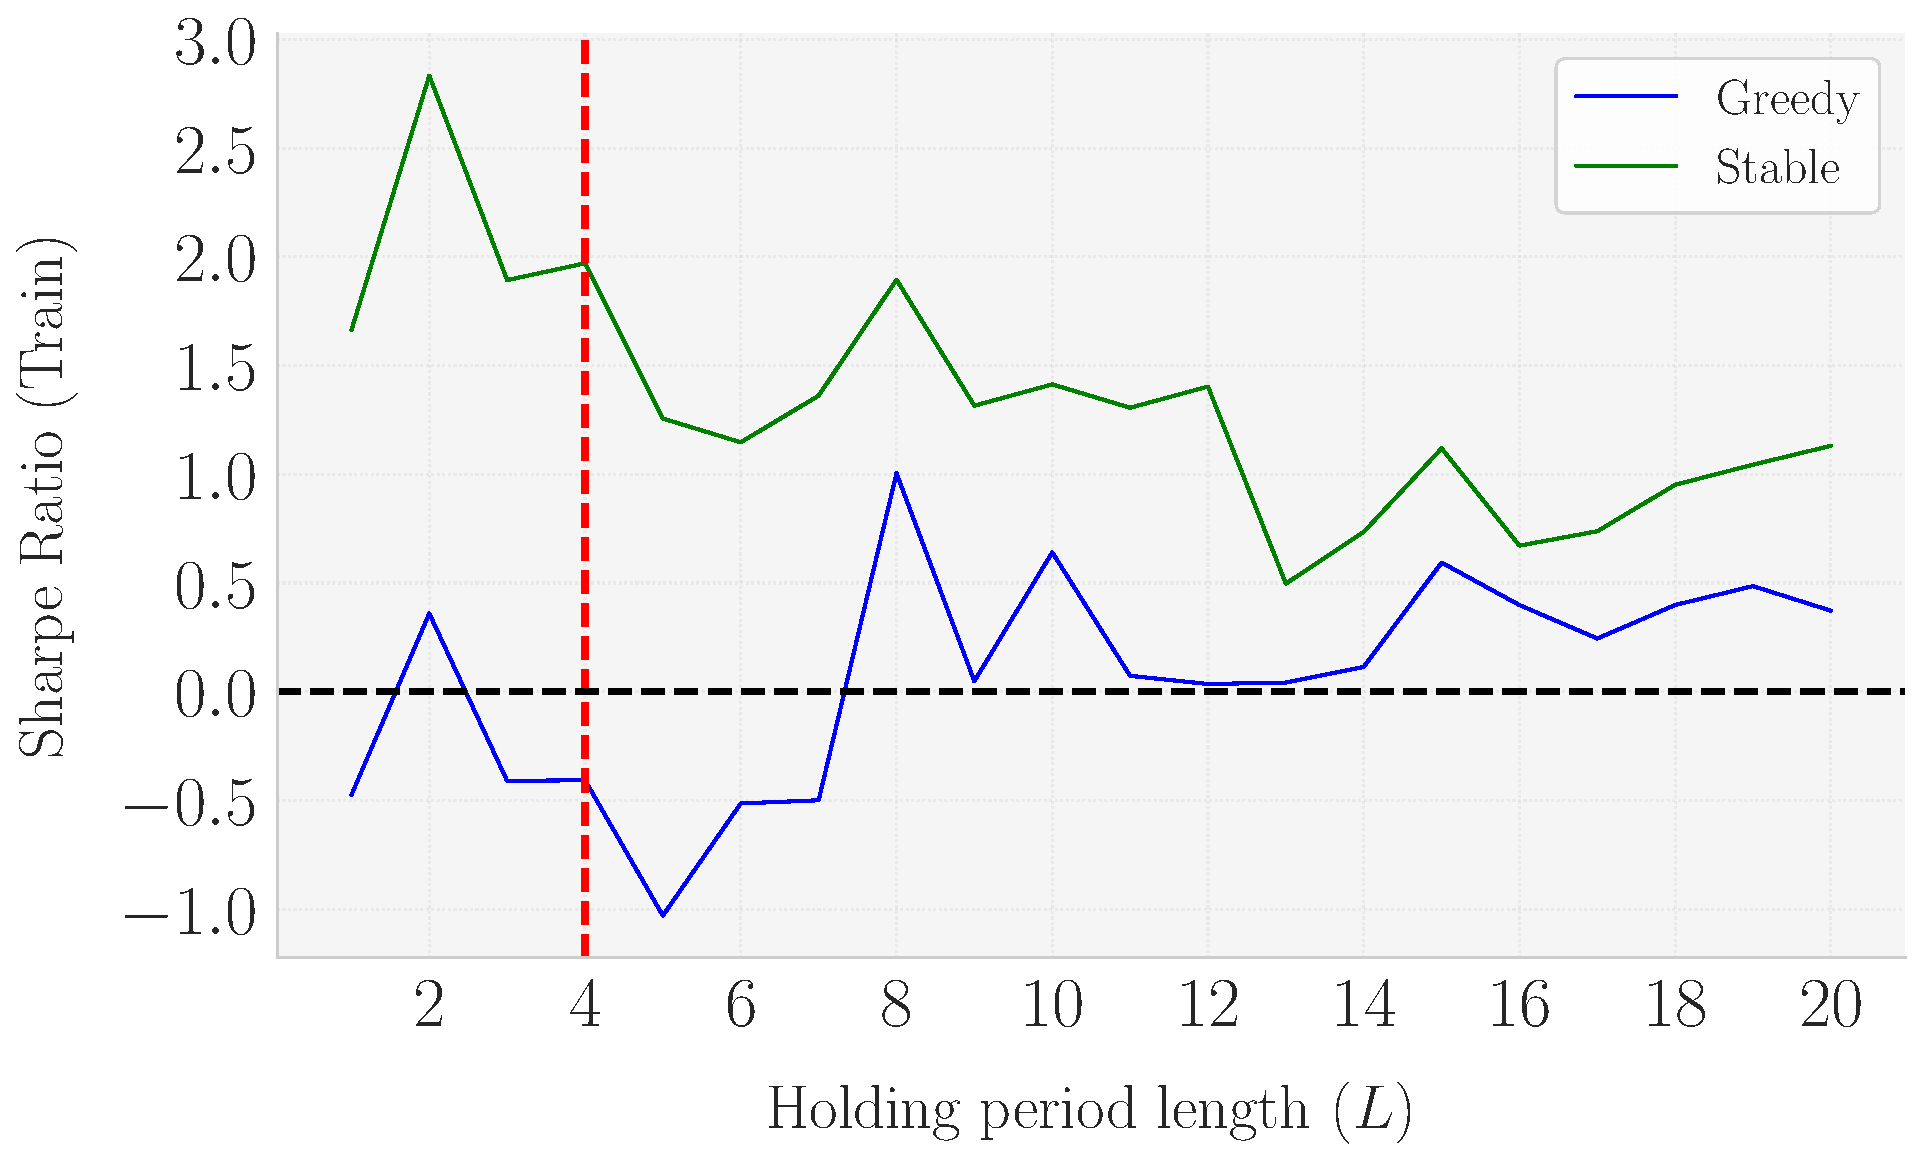
\includegraphics[width=\textwidth]{/Users/jesusvillotamiranda/Library/CloudStorage/OneDrive-UniversidaddeLaRioja/CEMFI/__MSc__/__Second_year__/6th_Term/MasterThesis/__Output/KMeans_RobustnessCheck_SR_Train_Set_vs_L_[Change_L].pdf}
    \caption{Plot of $SR^{\mathcal P^{tr}}(L)$ over a grid of $L$}
    \label{fig:K_hyp_1}
  \end{subfigure}
  \hspace{0.05\textwidth} % Add horizontal space between the subfigures
  \begin{subfigure}[b]{0.46\textwidth}
    \centering
    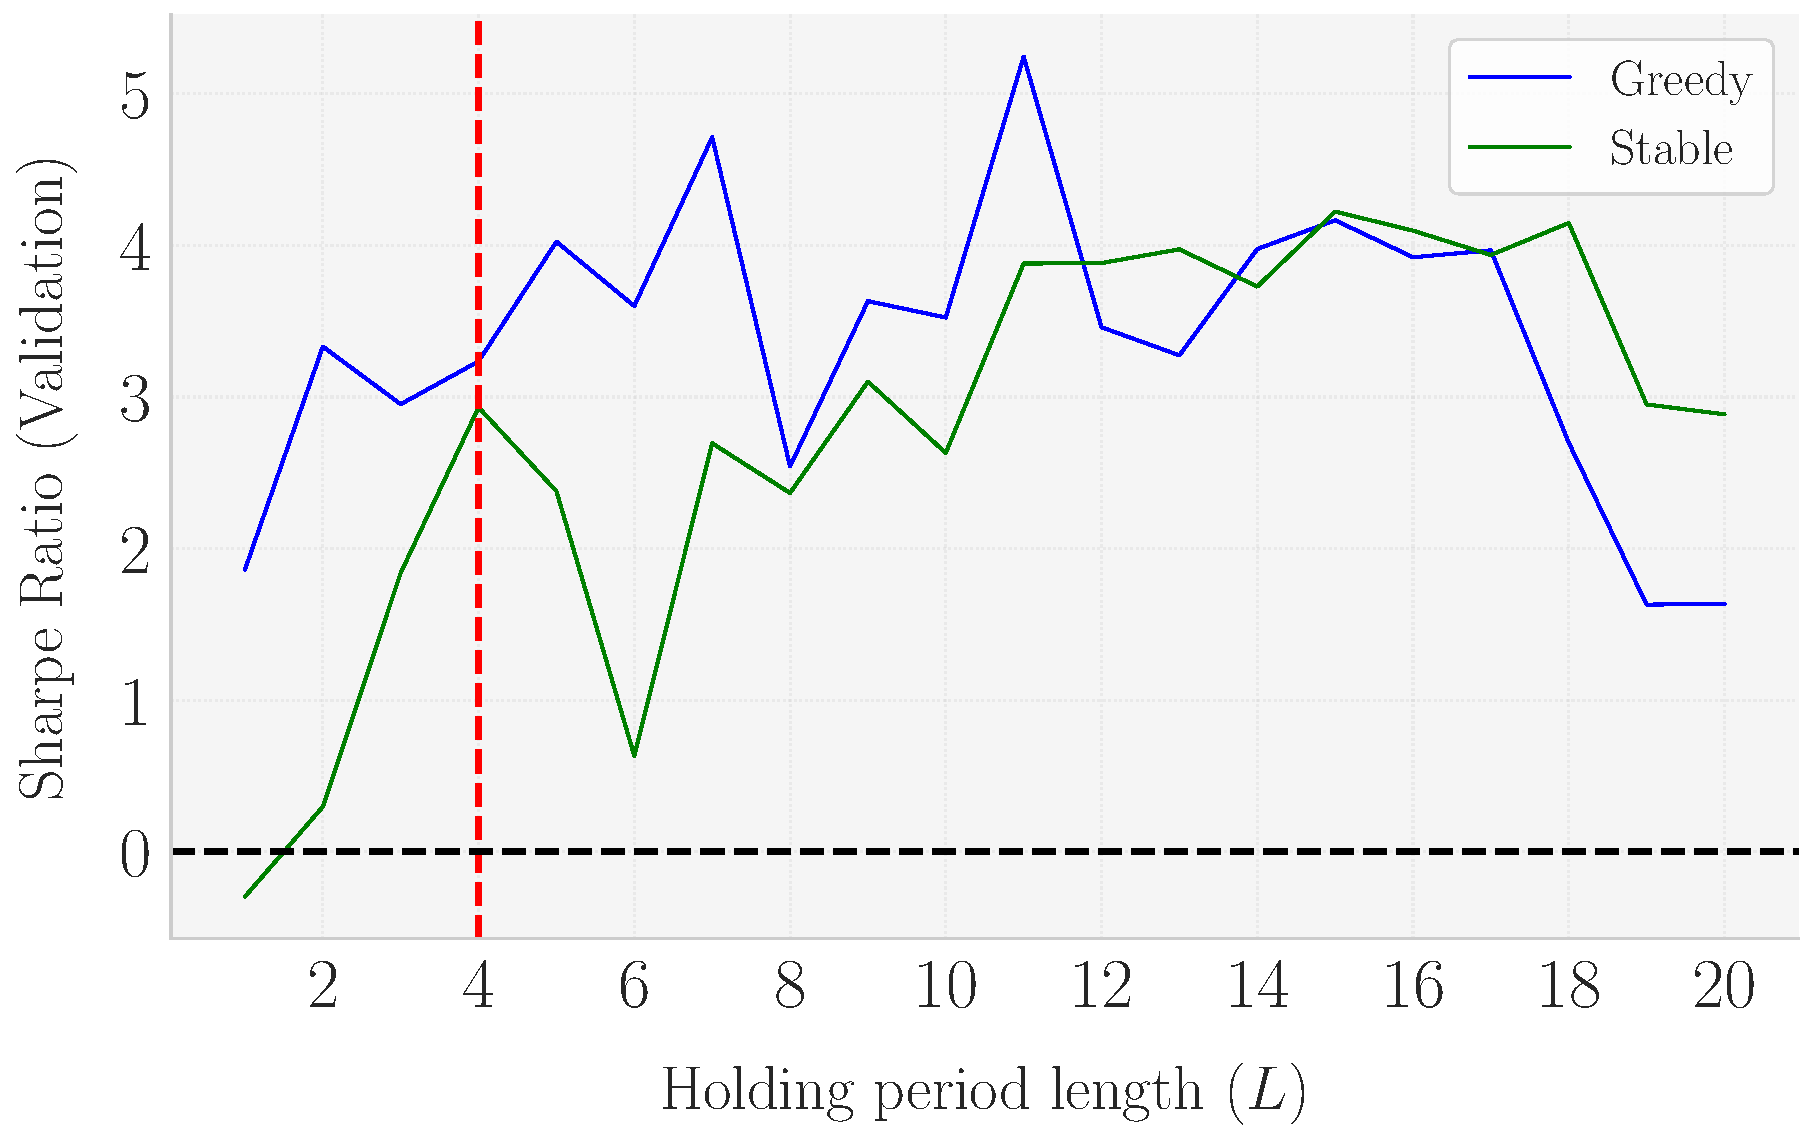
\includegraphics[width=\textwidth]{/Users/jesusvillotamiranda/Library/CloudStorage/OneDrive-UniversidaddeLaRioja/CEMFI/__MSc__/__Second_year__/6th_Term/MasterThesis/__Output/KMeans_RobustnessCheck_SR_Validation_Set_vs_L_[Change_L].pdf}
    \caption{Plot of $SR^{\mathcal P^{val}}(L)$ over a grid of $L$}
    \label{fig:K_hyp_2}
  \end{subfigure}  
  \mx
  \subcaption*{\textit{Note: This figure shows the Sharpe Ratios ($SR$) as a function of the holding period length ($L$) for the KMeans clustering method in the training (Panel a) and validation (Panel b) splits. In Panel (a), the Sharpe Ratios in the training set indicate that lower values of $L$ (less than 4) maximize performance. Conversely, in Panel (b), the validation set shows higher Sharpe Ratios for longer holding periods. The choice of $L=4$ represents a balanced compromise, providing a stable Sharpe Ratio profile across both splits, ensuring consistent in-sample performance without introducing lookahead bias.}}
  \label{fig:KMeans_hyperparameter_justification_L}
\end{figure}
%----------------------------------------------------

On the other hand, the choice of $\theta=\integer{0.5\cd 26}=13$ is a choice that pursues stability in the Sharpe Ratio of the train and validation portfolios. As we can see from \cref{fig:KMeans_hyperparameter_justification_theta}, the Sharpe Ratios tend to converge to the highest and most stable value when we choose the highest possible value of $\theta$. 

 %----------------------------------------------------
\inserthere{fig:KMeans_hyperparameter_justification_theta}
\begin{figure}[H]
  \caption{Sharpe Ratios in the train and validation splits as a function of $\theta$ (KMeans)}
  \centering
    \begin{subfigure}[b]{0.46\textwidth}
    \centering
    \includegraphics[width=\textwidth]{/Users/jesusvillotamiranda/Library/CloudStorage/OneDrive-UniversidaddeLaRioja/CEMFI/__MSc__/__Second_year__/6th_Term/MasterThesis/__Output/KMeans_RobustnessCheck_SR_Train_Set_vs_theta_[Change_theta].pdf}
    \caption{Plot of $SR^{\mathcal P^{tr}}(\theta)$ over a grid of $\theta$}
    \label{fig:K_hyp_3}
  \end{subfigure}
  \hspace{0.05\textwidth} % Add horizontal space between the subfigures
  \begin{subfigure}[b]{0.46\textwidth}
    \centering
    \includegraphics[width=\textwidth]{/Users/jesusvillotamiranda/Library/CloudStorage/OneDrive-UniversidaddeLaRioja/CEMFI/__MSc__/__Second_year__/6th_Term/MasterThesis/__Output/KMeans_RobustnessCheck_SR_Validation_Set_vs_theta_[Change_theta].pdf}
    \caption{Plot of $SR^{\mathcal P^{val}}(\theta)$ over a grid of $\theta$}
    \label{fig:K_hyp_4}
  \end{subfigure}
  \mx
\subcaption*{\textit{Note: This figure illustrates the Sharpe Ratios ($SR$) as a function of $\theta$, the upper bound on the number of traded clusters, for the KMeans clustering method in the training (Panel a) and validation (Panel b) splits. In Panel (a), the Sharpe Ratios in the training set show a trend of increasing stability and maximizing performance as $\theta$ approaches its upper limit. Similarly, Panel (b) displays a consistent pattern in the validation set, where higher values of $\theta$ lead to convergence at the highest and most stable Sharpe Ratios. The choice of $\theta = 13$ (i.e: $\integer{0.5 \cdot 26}$) reflects this observed stability and optimization, providing a balanced and robust selection for the portfolio strategy.}}
  \label{fig:KMeans_hyperparameter_justification_theta}
\end{figure}
%----------------------------------------------------


\subsubsection{LLM Clustering}
Following a similar logic as below, the choice of $L=4$ sets a consensus between the maximization of $SR^{\mathcal P^{tr}}$ and $SR^{\mathcal P^{val}}$. That is, maximizing $SR^{\mathcal P^{tr}}$ requires lower holding period lengths (the maximizer is $L=4$), while maximizing $SR^{\mathcal P^{val}}$ requires increasing the window length. Among this contradiction, $L=4$ standing as a perfect choice to balance the maximization requirements in both samples, generating a stable choice for the holding period window length.

%----------------------------------------------------
\inserthere{fig:LLM_hyperparameter_justification_L}
\begin{figure}[H]
  \caption{Sharpe Ratios in the train and validation splits as a function of hyperparameters (LLM)}
  \centering
  
  \begin{subfigure}[b]{0.46\textwidth}
    \centering
    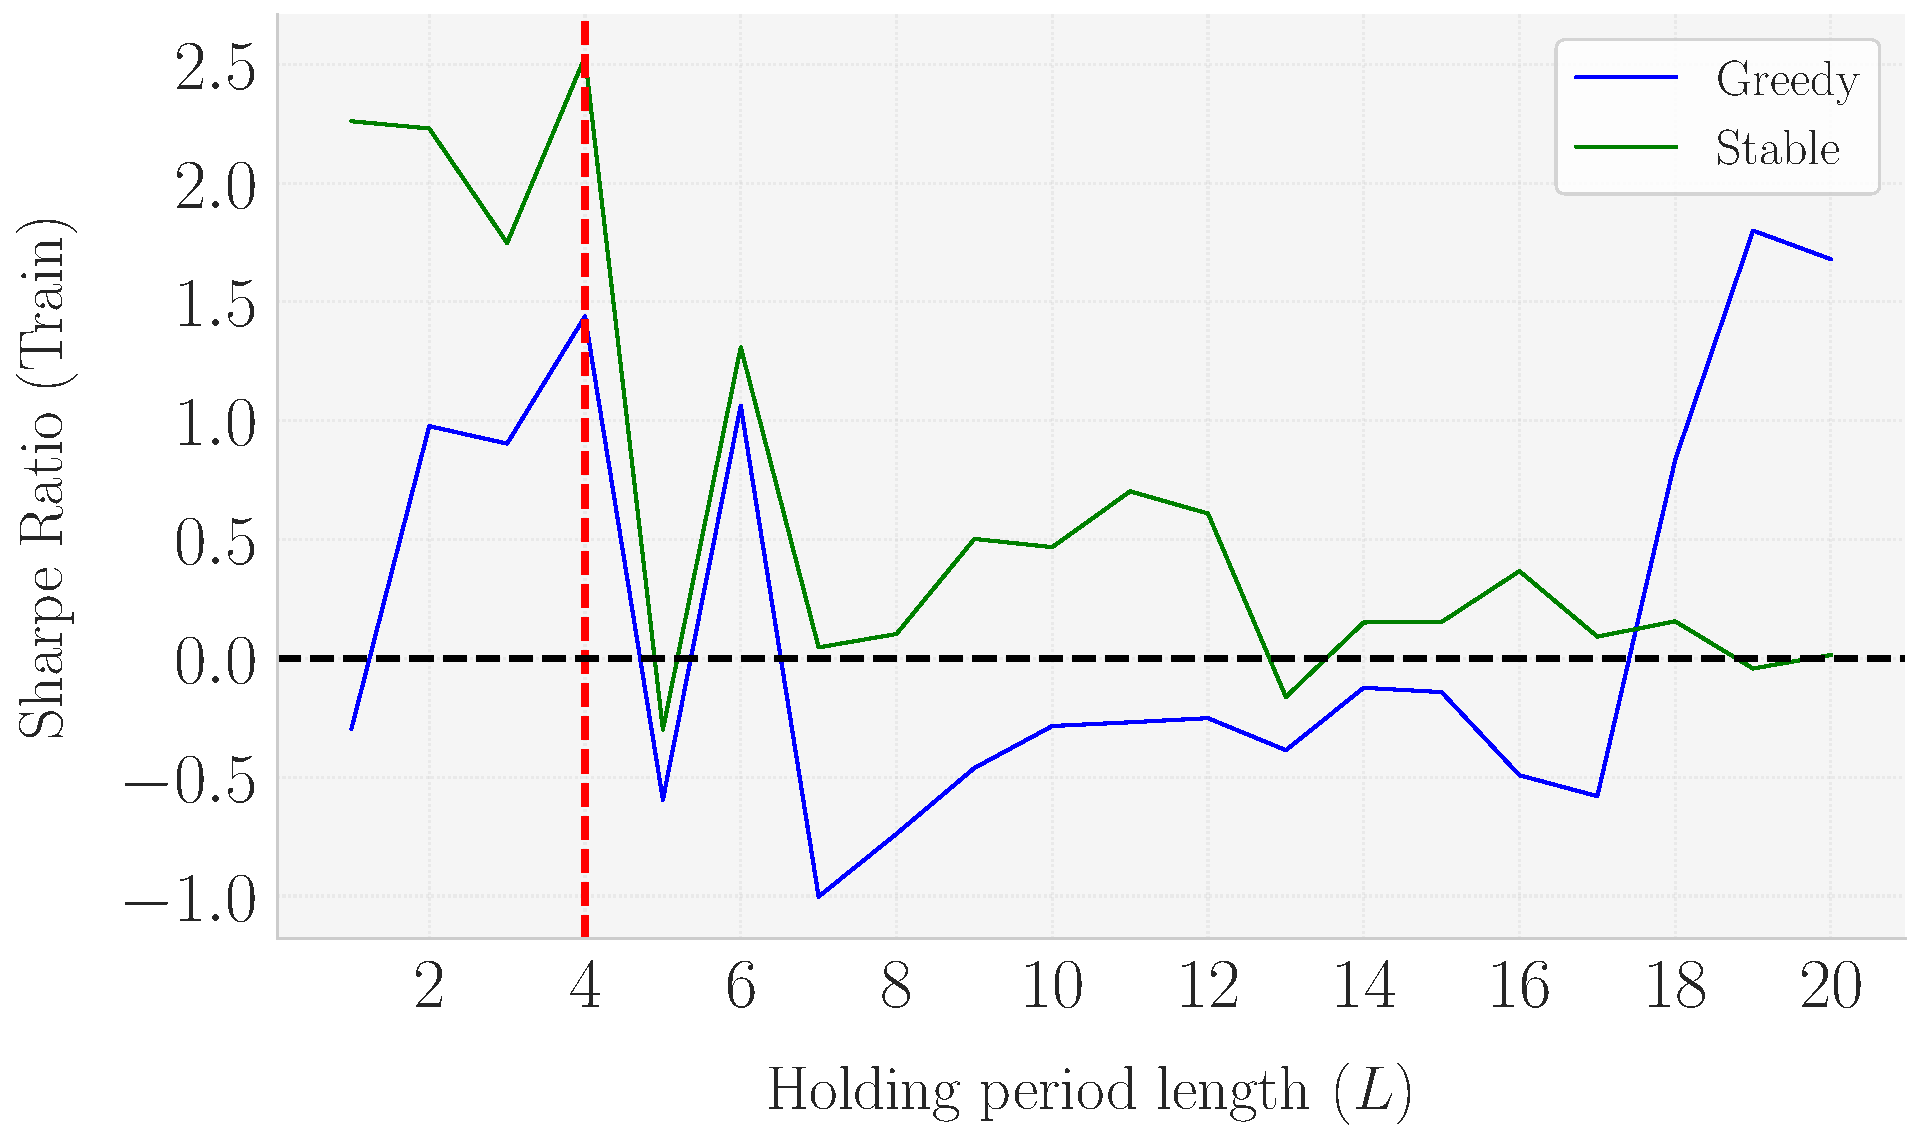
\includegraphics[width=\textwidth]{/Users/jesusvillotamiranda/Library/CloudStorage/OneDrive-UniversidaddeLaRioja/CEMFI/__MSc__/__Second_year__/6th_Term/MasterThesis/__Output/LLAMA_RobustnessCheck_SR_Train_Set_vs_L_[Change_L].pdf}
    \caption{Plot of $SR^{\mathcal P^{tr}}(L)$ over a grid of $L$}
    \label{fig:LLM_hyp_1}
    
  \end{subfigure}
  \hspace{0.05\textwidth} % Add horizontal space between the subfigures
  \begin{subfigure}[b]{0.46\textwidth}
    \centering
    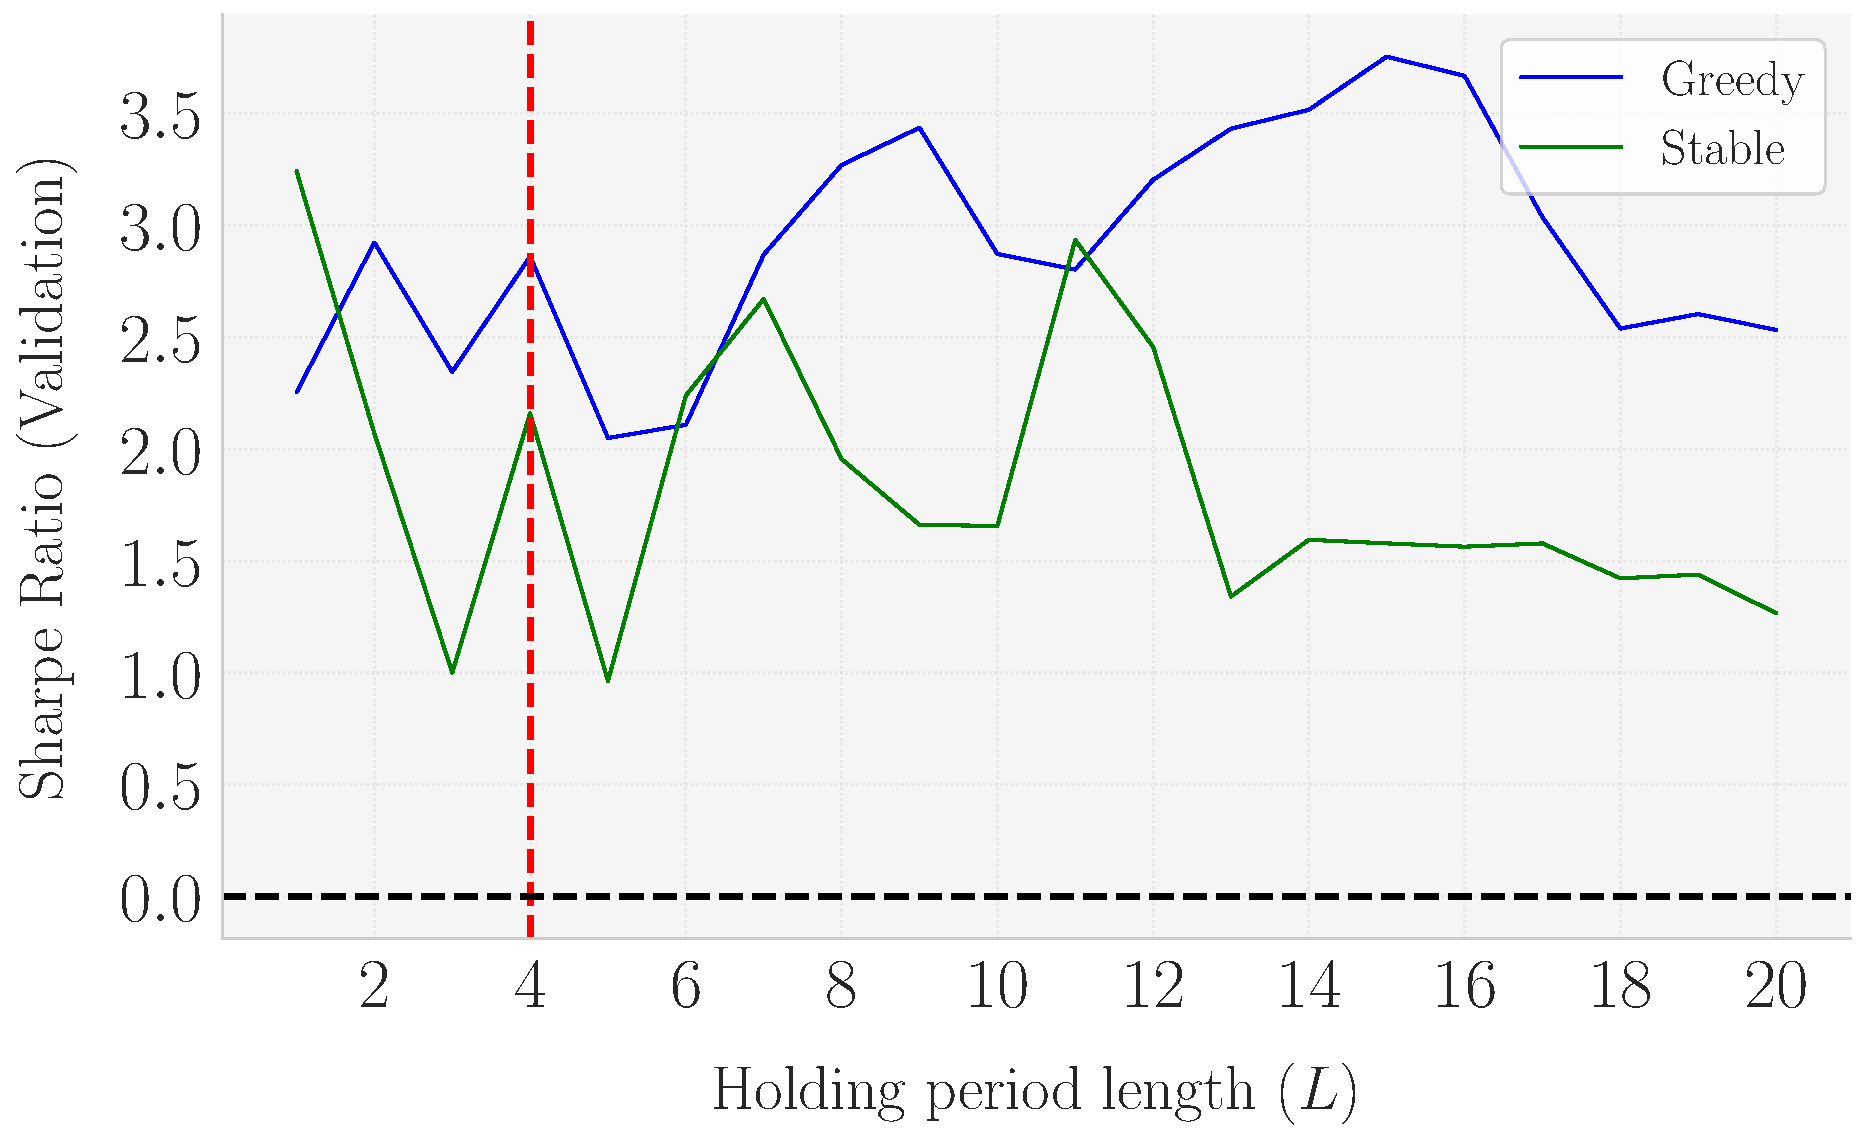
\includegraphics[width=\textwidth]{/Users/jesusvillotamiranda/Library/CloudStorage/OneDrive-UniversidaddeLaRioja/CEMFI/__MSc__/__Second_year__/6th_Term/MasterThesis/__Output/LLAMA_RobustnessCheck_SR_Validation_Set_vs_L_[Change_L].pdf}
    \caption{Plot of $SR^{\mathcal P^{val}}(L)$ over a grid of $L$}
    \label{fig:LLM_hyp_2}
  \end{subfigure}
  \mx 
  \subcaption*{\textit{Note: This figure shows the Sharpe Ratios ($SR$) as a function of the holding period length ($L$) for the LLM clustering method, across the training (Panel a) and validation (Panel b) splits. In Panel (a), the Sharpe Ratios in the training set reach their maximum at $L=4$, suggesting shorter holding periods are more effective for maximizing performance. Conversely, Panel (b) illustrates that longer holding periods yield higher Sharpe Ratios in the validation set. The choice of $L=4$ serves as a compromise, balancing the trade-off between maximizing $SR$ in both splits and providing a stable and consistent holding period length for the strategy.}}
  \label{fig:LLM_hyperparameter_justification_L}
\end{figure}
%----------------------------------------------------

Finally, the same conclusion as in KMeans applies here. By selecting $\theta=\integer{0.5\cd 20}=10$, we get a stable Sharpe Ratio. Even though we observe that $SR^{\mathcal P^{tr}}(L)$ falls momentarily at $\theta=10$ for the Greedy algorithm, it still constitutes a good choice. Conversely, at $\theta=10$ the greedy algorithm sees a jump in $SR^{\mathcal P^{val}}(L)$. All in all, we can easily conclude that $\theta=\integer{0.5k}$ arises as a good hyperpamrameter choice also for LLM clustering.
%----------------------------------------------------
\inserthere{fig:LLM_hyperparameter_justification_theta}
\begin{figure}[H]
\caption{Sharpe Ratios in the train and validation splits as a function of $\theta$ (LLM)}
  \centering

    \begin{subfigure}[b]{0.46\textwidth}
    \centering
    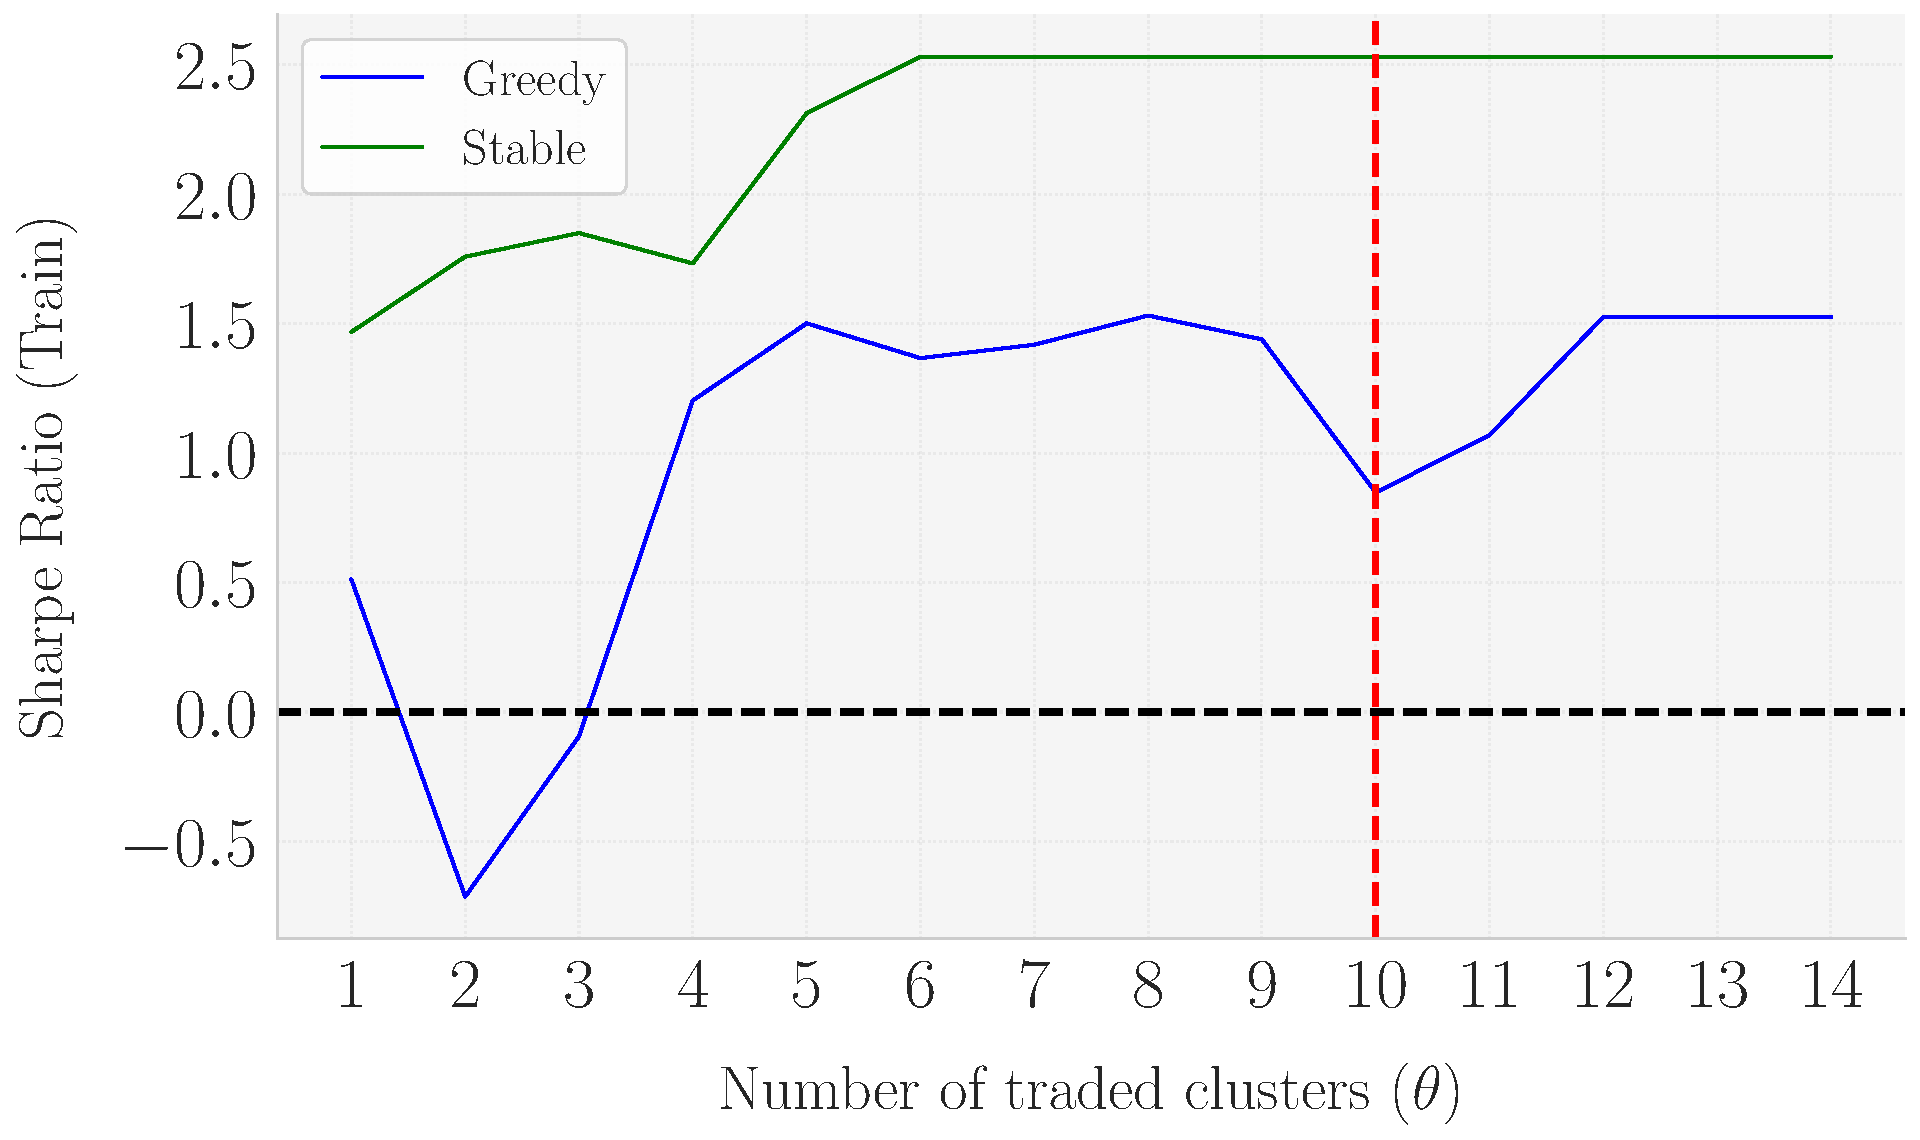
\includegraphics[width=\textwidth]{/Users/jesusvillotamiranda/Library/CloudStorage/OneDrive-UniversidaddeLaRioja/CEMFI/__MSc__/__Second_year__/6th_Term/MasterThesis/__Output/LLAMA_RobustnessCheck_SR_Train_Set_vs_Theta_[Change_theta].pdf}
    \caption{Plot of $SR^{\mathcal P^{tr}}(\theta)$ over a grid of $\theta$}
    \label{fig:LLM_hyp_3}
  \end{subfigure}
  \hspace{0.05\textwidth} % Add horizontal space between the subfigures
  \begin{subfigure}[b]{0.46\textwidth}
    \centering
    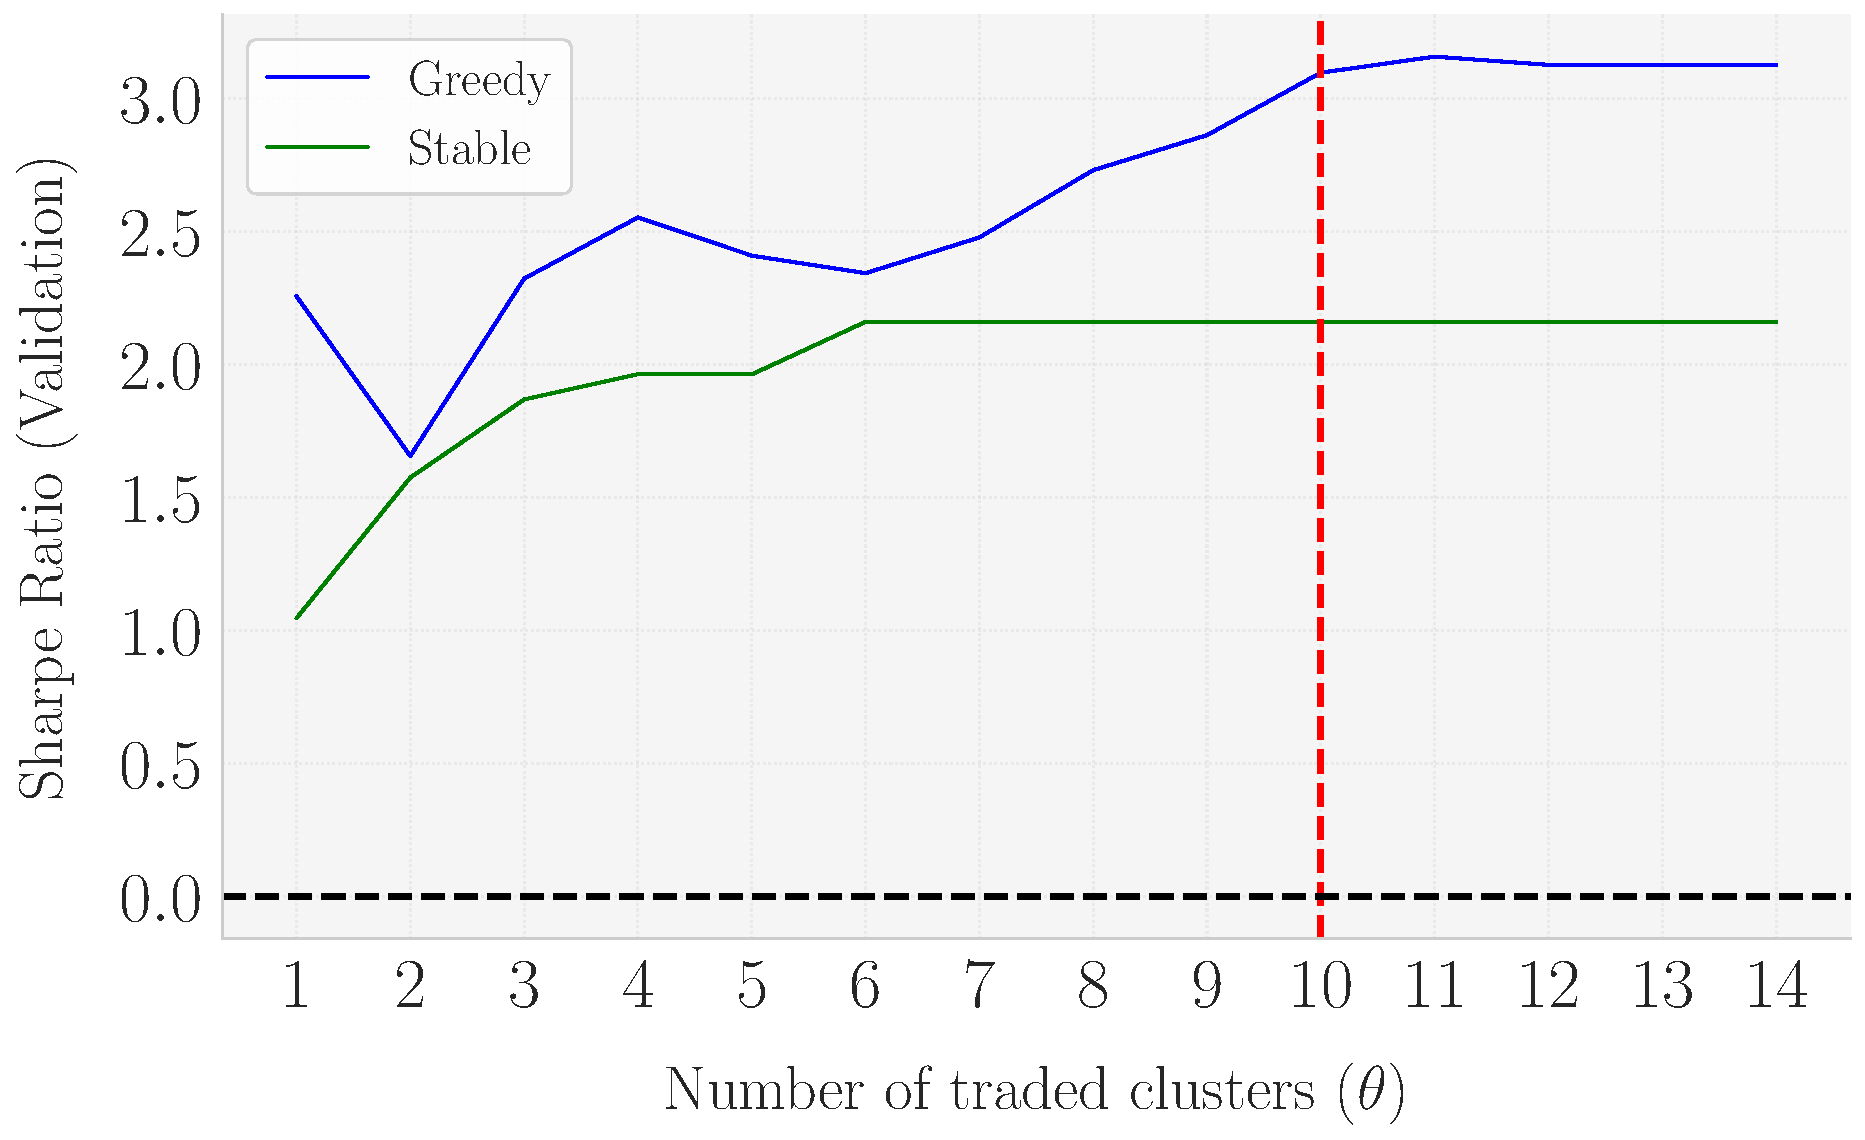
\includegraphics[width=\textwidth]{/Users/jesusvillotamiranda/Library/CloudStorage/OneDrive-UniversidaddeLaRioja/CEMFI/__MSc__/__Second_year__/6th_Term/MasterThesis/__Output/LLAMA_RobustnessCheck_SR_Validation_Set_vs_Theta_[Change_theta].pdf}
    \caption{Plot of $SR^{\mathcal P^{val}}(\theta)$ over a grid of $\theta$}
    \label{fig:LLM_hyp_4}
  \end{subfigure}
\mx
\subcaption*{\textit{Note: This figure illustrates the Sharpe Ratios ($SR$) as a function of $\theta$, the upper bound on the number of traded clusters, for the LLM clustering method in the training (Panel a) and validation (Panel b) splits. In Panel (a), the Sharpe Ratios for the training set indicate a temporary dip at $\theta=10$ for the Greedy algorithm, yet this value still provides a relatively stable outcome. In contrast, Panel (b) shows that $\theta=10$ leads to a noticeable increase in Sharpe Ratios for the validation set, particularly benefiting the Greedy algorithm. The choice of $\theta = \integer{0.5k} = 10$ strikes a balance, confirming it as an effective hyperparameter selection for achieving stability in both the training and validation splits with LLM clustering.}}
\label{fig:LLM_hyperparameter_justification_theta}
\end{figure}
%----------------------------------------------------


%%%%%%%%%%%%%%%%%%%%%%%%%%%%%%%%%%%%%%%%%%%%%%%%%%%%%

\newpage
%%%%%%%%%%%%%%%%%%%%%%%%%%%%%%%%%%%%%%%%%%%%%%%%%%%%%
\subsection{Optimal Cluster Selection Algorithms}
%%%%%%%%%%%%%%%%%%%%%%%%%%%%%%%%%%%%%%%%%%%%%%%%%%%%%
%----------------------------------------------------
\begin{algorithm}
\caption{
\textsc{Greedy Selection} 
~|~
{{Top average Sharpe Ratio in Validation Set}}
}
%%%%%%%%%%%%%%%%%%%%%%%%%%%%%%%%%%%%%%%%%%%%%%%%%%%%%
\label{alg:greedy_selection}
%%%%%%%%%%%%%%%%%%%%%%%%%%%%%%%%%%%%%%%%%%%%%%%%%%%%%
\begin{algorithmic}[1]
\mx 
\State \textbf{Input:} Set of clusters $\mathcal{G} = \{1, 2, \ldots, k^*\}$, Sharpe Ratios in the validation sample $\{SR_L^{(i,j)}\}_{(i,j)\in \mathcal B^{val}}$, maximum number of traded clusters $\theta\in\mathbb{N}$ (usually, $\theta\propto k^*)$

\mx 
\State \textbf{Output:} Set of long-traded clusters $\mathcal{G}_{\theta}^{+}$ and set of short-traded clusters $\mathcal{G}_{\theta}^{-}$
%----------------------------------------------------
%\Statex
\vspace{0.4cm}
\Statex \underline{\textit{Step \#1: Compute Cluster Average Sharpe Ratios in Validation Set}}
\For{each $g \in \mathcal{G}$}
    \State Compute average Sharpe Ratio ~
$
\overline{S R}_g^{val} \leftarrow \frac{1}{|\mathcal{B}_g^{val} |} \sum_{(i,j) \in \mathcal{B}_g^{val}} S R_{{{L}}}^{(i,j)}
$
\EndFor
%----------------------------------------------------
%\Statex
\vspace{0.4cm}
\Statex \underline{\textit{Step \#2: Identify Positive and Negative Sharpe Ratio Clusters}}
\State Define $\mathcal{G}_{SR^+}^{val} \leftarrow \{ g \in \mathcal{G} \mid \overline{SR}_g^{val} > 0 \}$
\State Define $\mathcal{G}_{SR^-}^{val} \leftarrow \{ g \in \mathcal{G} \mid \overline{SR}_g^{val} < 0 \}$
%----------------------------------------------------
\vspace{0.4cm}
\Statex \underline{\textit{Step \#3: Rank Clusters by Average Sharpe Ratio in the Validation Set}}
\For{each $g \in \mathcal{G}$}
	\State Rank the average Sharpe Ratio~~
$
\mathfrak{R}_g^{val} \leftarrow  \sum_{h \in \mathcal{G}} 
\mathbf{1}\1{
\overline{S R}_h^{val} \geq \overline{S R}_g^{val} 
}
$
\EndFor
%\State Sort clusters in descending order of $\overline{SR}_g^{val}$
%%\State
%$$\overline{SR}_{\varkappa_1}^{val} \geq \overline{SR}_{\varkappa_2}^{val} \geq \ldots \geq \overline{SR}_{\varkappa_{k^*}}^{val}$$
%----------------------------------------------------
%\Statex
\vspace{0.4cm}
\Statex \underline{\textit{Step \#4: Select Top $\theta$ Clusters}}
\State Define $\theta^+ \leftarrow \min(\theta, |\mathcal{G}_{SR^+}^{val}|)$
;~~
$\mathcal{G}_{\theta}^{+} \leftarrow \{ g\in\G \mid 1 \leq \mathfrak{R}_g^{val} \leq \theta^+ \}$
%\State 

\State Define $\theta^- \leftarrow \min(\theta, |\mathcal{G}_{SR^-}^{val}|)$
;~~
%\State 
 $\mathcal{G}_{\theta}^{-} \leftarrow \{ g \in\G \mid k^* - \theta^- < \mathfrak{R}_g^{val} \leq k^* \}$
%----------------------------------------------------
%\Statex
\vspace{0.5cm}
\State \textbf{Return} Long-traded clusters $\mathcal{G}_{\theta}^{+}$, Short-traded clusters $\mathcal{G}_{\theta}^{-}$

\end{algorithmic}
\end{algorithm}


%
%\begin{algorithm}[H]
%\caption{Greedy Selection of Clusters Based on Average Sharpe Ratio}
%%%%%%%%%%%%%%%%%%%%%%%%%%%%%%%%%%%%%%%%%%%%%%%%%%%%%%
%\label{alg:greedy_selection}
%%%%%%%%%%%%%%%%%%%%%%%%%%%%%%%%%%%%%%%%%%%%%%%%%%%%%%
%\begin{algorithmic}[1]
%\State \textbf{Input:} Set of clusters $\mathcal{G} = \{1, 2, \ldots, k^*\}$, Sharpe Ratios in the validation sample $\{SR_L^{(i,j)}\}_{(i,j)\in \mathcal{B}^{val}}$, maximum number of traded clusters $\theta \in \mathbb{N}$ (usually, $\theta \propto k^*$)
%\State \textbf{Output:} Set of long-traded clusters $\mathcal{G}_{\theta}^{+}$ and set of short-traded clusters $\mathcal{G}_{\theta}^{-}$
%
%\Statex
%\Statex \underline{\textit{Step \#1: Compute Cluster Average Sharpe Ratios in Validation Set}}
%\For{each $g \in \mathcal{G}$}
%    \State Compute average Sharpe Ratio ~
%    \[
%    \overline{SR}_g^{val} \leftarrow \frac{1}{|\mathcal{B}_g^{val} |} \sum_{(i,j) \in \mathcal{B}_g^{val}} SR_{L}^{(i,j)}
%    \]
%\EndFor
%
%\Statex
%\Statex \underline{\textit{Step \#2: Identify Positive and Negative Sharpe Ratio Clusters}}
%\State Define $\mathcal{G}_{SR^+}^{val} \leftarrow \{ g \in \mathcal{G} \mid \overline{SR}_g^{val} > 0 \}$
%\State Define $\mathcal{G}_{SR^-}^{val} \leftarrow \{ g \in \mathcal{G} \mid \overline{SR}_g^{val} < 0 \}$
%
%\Statex
%\Statex \underline{\textit{Step \#3: Rank Clusters by Average Sharpe Ratio}}
%\State Sort clusters in descending order of $\overline{SR}_g^{val}$
%%\State
%\[
%\overline{SR}_{\varkappa_1}^{val} \geq \overline{SR}_{\varkappa_2}^{val} \geq \ldots \geq \overline{SR}_{\varkappa_{k^*}}^{val}
%\]
%
%\Statex
%\Statex \underline{\textit{Step \#4: Select Top $\theta$ Clusters}}
%\State Define $\theta^+ \leftarrow \min(\theta, |\mathcal{G}_{SR^+}^{val}|)$
%\State Define $\theta^- \leftarrow \min(\theta, |\mathcal{G}_{SR^-}^{val}|)$
%
%\State Define $\mathcal{G}_{\theta}^{+} \leftarrow \{ \varkappa_{\ell} \in \mathcal{G} \mid 1 \leq \ell \leq \theta^+ \}$
%\State Define $\mathcal{G}_{\theta}^{-} \leftarrow \{ \varkappa_{\ell} \in \mathcal{G} \mid k^* - \theta^- < \ell \leq k^* \}$
%
%\Statex
%\State \textbf{Return} Long-traded clusters $\mathcal{G}_{\theta}^{+}$, Short-traded clusters $\mathcal{G}_{\theta}^{-}$
%
%\end{algorithmic}
%\end{algorithm}

%----------------------------------------------------


%----------------------------------------------------
\begin{algorithm}[H]
\caption{
\textsc{Rank Stability}
~ |~
{{Minimal Rank Difference between Train \& Validation Sets}
}}
%%%%%%%%%%%%%%%%%%%%%%%%%%%%%%%%%%%%%%%%%%%%%%%%%%%%%
\label{alg:rank_stability}
%%%%%%%%%%%%%%%%%%%%%%%%%%%%%%%%%%%%%%%%%%%%%%%%%%%%%
\begin{algorithmic}[1]
\mx 
\State \textbf{Input:} Set of clusters $\mathcal{G} = \{1, 2, \ldots, k^*\}$, Sharpe Ratios in the training and validation sample $\{SR_L^{(i,j)}\}_{(i,j)\in \mathcal B^{tr}}$ and $\{SR_L^{(i,j)}\}_{(i,j)\in \mathcal B^{val}}$, maximum number of traded clusters $\theta$
\mx 
\State \textbf{Output:} Set of long-traded clusters $\mathcal{G}_{\theta}^{+}$ and set of short-traded clusters $\mathcal{G}_{\theta}^{-}$
%----------------------------------------------------
%\Statex
\mx
\Statex \underline{\textit{Step \#1: Compute Cluster Average Sharpe Ratios in Training \& Validation Set}}
\For{each $g \in \mathcal{G}$}
    \State Compute average Sharpe Ratio in $\mathcal B^{tr}:$ ~~
$
\overline{S R}_g^{tr} \leftarrow \frac{1}{|\mathcal{B}_g^{tr} |} \sum_{(i,j) \in \mathcal{B}_g^{tr}} S R_{{{L}}}^{(i,j)}
$
    \State Compute average Sharpe Ratio in $\mathcal B^{val}:$ ~
$
\overline{S R}_g^{val} \leftarrow \frac{1}{|\mathcal{B}_g^{val} |} \sum_{(i,j) \in \mathcal{B}_g^{val}} S R_{{{L}}}^{(i,j)}
$
\EndFor
%----------------------------------------------------
%\Statex
\mx
\Statex \underline{\textit{Step \#2: Rank Clusters}}
%\State \# \textit{Step 1: Rank Clusters}
\For{each $g \in \mathcal{G}$}
    \State Rank the average Sharpe Ratios in $\mathcal B^{tr}:$ ~~
%$\{\overline{S R}_g^{tr}\}_{g\in\G}$ 
$
\mathfrak{R}_g^{tr} \leftarrow  \sum_{h \in \mathcal{G}} 
\mathbf{1}\1{
\overline{S R}_h^{t r} \geq \overline{S R}_g^{t r} 
}
$
    \State Rank the average Sharpe Ratios in $\mathcal B^{val}:$ ~
%$\{\overline{S R}_g^{tr}\}_{g\in\G}$ 
$
\mathfrak{R}_g^{val} \leftarrow  \sum_{h \in \mathcal{G}} 
\mathbf{1}\1{
\overline{S R}_h^{val} \geq \overline{S R}_g^{val} 
}
$
\EndFor
%----------------------------------------------------
%\Statex
\mx
\Statex \underline{\textit{Step \#3: Calculate Rank Differences}}
\For{each $g \in \mathcal{G}$}
    \State Calculate rank difference $\delta_g \leftarrow | \mathfrak R_g^{tr} - \mathfrak R_g^{val} |$
\EndFor
%----------------------------------------------------
%\Statex
\mx
\Statex \underline{\textit{Step \#4: Select Top $\theta$ Clusters with Smallest Rank Differences}}
\For{each $g \in \mathcal{G}$}
\State Rank the rank difference $:~~ \mathfrak{R}(\delta_g) \leftarrow \sum_{h\in\G} \mbf{1} \1{ \delta_g \geq  \delta_h }$
\EndFor
\State Select top $2\theta$ clusters with smallest $\delta_g$: 
$
~~
\mathcal{G}_{\theta} = 
\3{
g\in\G \c 1 \leq \mathfrak{R}(\delta_g) \leq 2\theta 
}
~
$
%----------------------------------------------------
%\Statex
\mx
\Statex \underline{\# \textit{Step 5: Determine Long and Short Positions}}
\State Define $\mathcal{G}_{\theta}^{+} = \{g \in \mathcal{G}_{\theta} \mid \overline{SR}_g^{tr} > 0 \text{ and } \overline{SR}_g^{val} > 0\}$
\State Define $\mathcal{G}_{\theta}^{-} = \{g \in \mathcal{G}_{\theta} \mid \overline{SR}_g^{tr} < 0 \text{ and } \overline{SR}_g^{val} < 0\}$
%----------------------------------------------------
%\Statex
\mx
\State \textbf{Return} Long-traded clusters $\mathcal{G}_{\theta}^{+}$, Short-traded clusters $\mathcal{G}_{\theta}^{-}$

\end{algorithmic}
\end{algorithm}


%----------------------------------------------------




%%%%%%%%%%%%%%%%%%%%%%%%%%%%%%%%%%%%%%%%%%%%%%%%%%%%%
\subsection{Sample of articles for each cluster}
%%%%%%%%%%%%%%%%%%%%%%%%%%%%%%%%%%%%%%%%%%%%%%%%%%%%%
\setcounter{table}{0}
\renewcommand{\thetable}{A\arabic{table}} % To ensure the tables in the appendix are numbered as A1, A2, etc.

%%----------------------------------------------------
%%%%%%%%%%%%%%%%%%%%%%%%%%%%%%%%%%%%%%%%%%%%%%%%%%%%%
%%%%%%%%%%%%%% 		ENGLISH 		%%%%%%%%%%%%%%%%%
%%%%%%%%%%%%%%%%%%%%%%%%%%%%%%%%%%%%%%%%%%%%%%%%%%%%%
%%%%%%%%%%%%%%%%%%%%%%%%%%%%%%%%%%%%%%%%%%%%%%%%%%%%%

\begin{landscape}
\renewcommand{\arraystretch}{1}

%\scriptsize
{\fontsize{9}{9}\selectfont % Set custom font size between \scriptsize and \tiny

%----------------------------------------------------
\begin{longtable}{|c|L{8cm}|L{14cm}|}
\caption{KMeans clustering. Proposed name for the clusters and sample of 3 articles for each cluster.} % Caption for the longtable
\label{tab:KMeans_Articles_3_English} \\
\hline 
\rowcolor{lightgray}
\# & \multicolumn{1}{c|}{Title} & \multicolumn{1}{c|}{Articles} \\
\hline \hline 
0 
& 
Miscellaneous (Colonial, Acciona, Amadeus, Grifols, Endesa, IAG, Bankinter...)
& 
\textbullet~Colonial forecasts rental income of EUR338m in 2020

\textbullet~Acciona's asset sales will allow it to grow in renewables

\textbullet~Sabadell recommends selling Amadeus shares due to worse sales forecast.
\\ \hline 
1
& 
Quarterly \& Semi-Annual Earnings Reports
& 
\textbullet~Enag�s 1H net profit falls 9.8\% due to lower income and extraordinary items.

\textbullet~Iberdrola: Net profit of EUR1.025m in Q1

\textbullet~Santander almost quintuples Q1 profit due to absence of Covid provisions.
\\ \hline 
2
& 
BBVA \& Sabadell: Financial Performance \& Strategic Movements
& 
\textbullet~Interest rate hike in Turkey favors BBVA's net interest margin

\textbullet~Sabadell reorganizes business in Spain following the arrival of the new CEO.

\textbullet~Fitch downgrades Banco Sabadell's rating one notch to low grade.
\\ \hline 
3
& 
Telef�nica \& Cellnex: Telecommunications Tower Sales \& Market Dynamics
& 
\textbullet~Telef�nica shares soar after selling towers of its subsidiary in Europe and Latin America.

\textbullet~Telef�nica hires Goldman Sachs to sell its British tower business

\textbullet~Dutch Competition Authority authorizes Cellnex to integrate 3,150 Deutsche Telekom towers.
\\ \hline 
4
& 
CaixaBank: Mergers and Strategic Moves in the Banking Sector
& 
\textbullet~CaixaBank and Bankia approve their merger project

\textbullet~CaixaBank closes its first issuance of green bonds in pounds for 500 million

\textbullet~CaixaBank-Bankia merger could generate EUR500m in savings
\\ \hline 
5
& 
Telef�nica, Indra, \& M�sM�vil: Regulatory and Strategic Moves in Telecom
& 
\textbullet~Indra to partner with Telef�nica in the deployment of fiber optics in Germany.

\textbullet~Telef�nica launches a buyback offer for its hybrid bonds of EUR1.000m.

\textbullet~EU refers Liberty Global and Telef�nica agreement to UK regulator
\\ \hline 
6
& 
Siemens Gamesa: Supply Agreements, Profitability Targets in Renewable Energy
& 
\textbullet~Siemens Gamesa will supply turbines to Elawan's 150 MW wind farm in Spain.

\textbullet~Siemens Gamesa lowers its profitability target for 2021.

\textbullet~Siemens Gamesa will supply 160 MW for the largest wind farm in the Philippines.
\\ \hline 
7
& 
Cellnex: Strategic Acquisitions and Financial Moves in Telecom Infrastructure
& 
\textbullet~Cellnex launches a EUR1.850m debt issue

\textbullet~Cellnex agrees to buy 10,500 telecommunications towers in France for EUR5.200m

\textbullet~Benetton family sells 2.5\% of Cellnex to Singapore sovereign fund
\\ \hline 
8
& 
Acciona, Endesa, Enag�s \& Naturgy: Strategic Moves \& Regulatory Developments in the Energy Sector
& 
\textbullet~Naturgy and Enag�s study project to produce green hydrogen in Asturias

\textbullet~Break of ties between Algeria and Morocco may damage gas flow to Spain

\textbullet~Acciona: Energy business IPO on track for 1H
\\ \hline 
9
& 
Repsol: Strategic Moves and Challenges in the Energy Sector
& 
\textbullet~Repsol to produce green hydrogen at Petronor refinery in 2022

\textbullet~Repsol and Talgo to jointly promote the creation of renewable hydrogen trains

\textbullet~Repsol gains access to a portfolio of renewable assets in Chile through a joint venture
\\ \hline 
10
& 
Ferrovial, Acciona: Strategic Expansions and Financial Maneuvers in Infrastructure
& 
\textbullet~Ferrovial closes the sale of Broadspectrum to Ventia for EUR291m

\textbullet~Acciona awarded the construction of 2 roads in Poland for EUR642m

\textbullet~Renfe awards on-board services contract to Ferrovial for EUR272m
\\ \hline 
11
& 
Solaria: Strategic Moves and Market Challenges in Renewable Energy
& 
\textbullet~Solaria invests EUR220m in Europe's largest photovoltaic park.

\textbullet~Solaria will supply energy to Shell and Axpo with Europe's largest photovoltaic plant

\textbullet~Goldman Sachs downgrades Solaria recommendation after stock rise.
\\ \hline 
12
& 
Iberdrola: Strategic Collaborations and Renewable Energy Developments
& 
\textbullet~Iberdrola will build a self-consumption plant for Lactalis factory in Spain.

\textbullet~Iberdrola and Mapfre launch a renewable energy co-investment vehicle in Spain.

\textbullet~Iberdrola partners with Mitsubishi to decarbonize the industry.
\\ \hline 
13
& 
IAG: Financial Performance
& 
\textbullet~IAG Q3 results worse than expected

\textbullet~IAG burns cash faster than anticipated

\textbullet~IAG stock may be pricing in a second capital increase
\\ \hline 
14
& 
Santander \& CaixaBank: Financial Moves and Sustainability Initiatives 
& 
\textbullet~CaixaBank mobilizes EUR12.000m in sustainable financing in the first 9 months of 2020.

\textbullet~EIB and Banco Santander will inject EUR587m into Portuguese SMEs.

\textbullet~Banco Santander, leader in renewable project financing in 2020.
\\ \hline 
15
& 
ACS \& Acciona: Strategic Movements and Infrastructure Projects
& 
\textbullet~ACS and Acciona win contracts for new Australian airport worth EUR164m.

\textbullet~Acciona awarded 3 contracts to operate wastewater treatment plants in Sardinia for EUR210m.

\textbullet~ACS expects net profit to grow by around 30\% in 2021
\\ \hline 
16
& 
Telef�nica: Financial Performance and Strategic Moves
& 
\textbullet~Reduction in Telef�nica's debt will improve analysts' perception

\textbullet~Telef�nica's profit more than doubles in Q1 due to lower financial expenses.

\textbullet~Telef�nica, Am�rica M�vil and TIM buy the mobile network of Brazil's Oi.
\\ \hline 
17
& 
Meli� and Spanish Tourism Sector: Challenges Amidst the Pandemic
& 
\textbullet~Meli�: Spanish hotel sector faces another uncertain summer with cautious optimism.

\textbullet~Meli� claims EUR116m from the Spanish government for pandemic-related damages.

\textbullet~Meli�: Local Covid-19 lockdowns will continue to affect Meli�.
\\ \hline 
18
& 
Takeover Bids for Naturgy and M�sM�vil
& 
\textbullet~Australian fund IFM launches EUR5.000m bid for 22.69\% of Naturgy.

\textbullet~Polygon fund asks CNMV to review and alter the bid for M�sM�vil.

\textbullet~IFM accepts Spanish government conditions in partial bid for Naturgy.
\\ \hline 
19
& 
Naturgy: Financial Performance
& 
\textbullet~Naturgy presents "weak" 2020 results

\textbullet~Naturgy may revise its strategic plan upwards due to gas prices.

\textbullet~Bank of America sees upside potential for Naturgy based on fundamentals.
\\ \hline 
20
& 
PharmaMar, Grifols: Regulatory Approvals and Market Moves in the Pharmaceutical Sector
& 
\textbullet~EU court annuls European Commission's refusal to market PharmaMar drug.

\textbullet~Grifols starts issuing EUR2.000m bonds to buy Biotest.

\textbullet~PharmaMar announces approval of lurbinectedin for lung cancer in Australia.
\\ \hline 
21
& 
Repsol: Financial Performance
& 
\textbullet~Repsol: Net loss of EUR3.289m in 2020.

\textbullet~Repsol reports a loss of EUR711m in Q4 due to exploration and production provisions

\textbullet~Repsol posts a loss of EUR94m in Q3 due to provisions and lower refining margins.
\\ \hline 
22
& 
Aena: Financial Performance
& 
\textbullet~JPMorgan raises Aena's target price to EUR155 from EUR135.

\textbullet~Aena risks a revenue cut of up to EUR2.000m due to rents.

\textbullet~Aena loses EUR170.7m in 1H as passenger traffic plummets due to the pandemic.
\\ \hline 
23
& 
Enag�s, Endesa, Iberdrola, Red El�ctrica: Regulatory and Market Challenges in the Energy Sector
& 
\textbullet~Spanish electric utilities will remain under pressure in the stock market 

\textbullet~Spanish government measures are bad news for the electric sector.

\textbullet~Spain's electricity price closes February with a 52\% drop vs January
\\ \hline 
24
& 
BBVA, CaixaBank, Banco Sabadell: Layoffs and Restructuring
& 
\textbullet~CaixaBank proposes to unions a redundancy plan affecting 8,291 employees.

\textbullet~Banco Santander closes its redundancy plan with 3,572 voluntary exits and 19 dismissals 

\textbullet~Sabadell prepares an adjustment plan affecting 2,000 employees
\\ \hline 
25
& 
Inditex, Acerinox: Market Performance and Strategic Developments in the Post-Covid Context
& 
\textbullet~Inditex reopens 94\% of its stores worldwide after Covid-19 pandemic.

\textbullet~Sale of Nippon Steel in Acerinox is negative, but expected.

\textbullet~Inditex stock already prices in a strong business recovery.
\\ \hline 
\end{longtable}
%----------------------------------------------------
}

\end{landscape}


%%%%%%%%%%%%%%%%%%%%%%%%%%%%%%%%%%%%%%%%%%%%%%%%%%%%%%
%%%%%%%%%%%%%%%%%%%%%%%%%%%%%%%%%%%%%%%%%%%%%%%%%%%%%%
%%%%%%%%%%%%%%% 		ENGLISH 		%%%%%%%%%%%%%%%%%
%%%%%%%%%%%%%%%%%%%%%%%%%%%%%%%%%%%%%%%%%%%%%%%%%%%%%%
%%%%%%%%%%%%%%%%%%%%%%%%%%%%%%%%%%%%%%%%%%%%%%%%%%%%%%
%
%\begin{landscape}
%\renewcommand{\arraystretch}{1}
%
%
%%\scriptsize
%{\fontsize{9}{9}\selectfont % Set custom font size between \scriptsize and \tiny
%
%
%
%%----------------------------------------------------
%\begin{longtable}{|c|L{8cm}|L{14cm}|}
%\caption{KMeans clustering. Proposed name for the clusters and sample of 3 articles for each cluster.} \\ % Caption for the longtable
%\hline 
%\rowcolor{lightgray}
%\# & \multicolumn{1}{c|}{Title} & \multicolumn{1}{c|}{Articles} \\
%\hline \hline 
%0 
%& 
%Miscellaneous (Colonial, Acciona, Amadeus, Grifols, Endesa, IAG, Bankinter...)
%& 
%\textbullet~Colonial forecasts rental income of EUR338m in 2020
%
%\textbullet~Acciona's asset sales will allow it to grow in renewables
%
%\textbullet~Sabadell recommends selling Amadeus shares due to worse sales forecast.
%\\ \hline 
%1
%& 
%Quarterly \& Semi-Annual Earnings Reports
%& 
%\textbullet~Enag�s 1H net profit falls 9.8\% due to lower income and extraordinary items.
%
%\textbullet~Iberdrola: Net profit of EUR1.025m in Q1
%
%\textbullet~Santander almost quintuples Q1 profit due to absence of Covid provisions.
%\\ \hline 
%2
%& 
%BBVA \& Sabadell: Financial Performance \& Strategic Movements
%& 
%\textbullet~Interest rate hike in Turkey favors BBVA's net interest margin
%
%\textbullet~Sabadell reorganizes business in Spain following the arrival of the new CEO.
%
%\textbullet~Fitch downgrades Banco Sabadell's rating one notch to low grade.
%\\ \hline 
%3
%& 
%Telef�nica \& Cellnex: Telecommunications Tower Sales \& Market Dynamics
%& 
%\textbullet~Telef�nica shares soar after selling towers of its subsidiary in Europe and Latin America.
%
%\textbullet~Telef�nica hires Goldman Sachs to sell its British tower business
%
%\textbullet~Dutch Competition Authority authorizes Cellnex to integrate 3,150 Deutsche Telekom towers.
%\\ \hline 
%4
%& 
%CaixaBank: Mergers and Strategic Moves in the Banking Sector
%& 
%\textbullet~CaixaBank and Bankia approve their merger project
%
%\textbullet~CaixaBank closes its first issuance of green bonds in pounds for 500 million
%
%\textbullet~CaixaBank-Bankia merger could generate EUR500m in savings
%\\ \hline 
%5
%& 
%Telef�nica, Indra, \& M�sM�vil: Regulatory and Strategic Moves in Telecom
%& 
%\textbullet~Indra to partner with Telef�nica in the deployment of fiber optics in Germany.
%
%\textbullet~Telef�nica launches a buyback offer for its hybrid bonds of EUR1.000m.
%
%\textbullet~EU refers Liberty Global and Telef�nica agreement to UK regulator
%\\ \hline 
%6
%& 
%Siemens Gamesa: Supply Agreements, Profitability Targets in Renewable Energy
%& 
%\textbullet~Siemens Gamesa will supply turbines to Elawan's 150 MW wind farm in Spain.
%
%\textbullet~Siemens Gamesa lowers its profitability target for 2021.
%
%\textbullet~Siemens Gamesa will supply 160 MW for the largest wind farm in the Philippines.
%\\ \hline 
%7
%& 
%Cellnex: Strategic Acquisitions and Financial Moves in Telecom Infrastructure
%& 
%\textbullet~Cellnex launches a EUR1.850m debt issue
%
%\textbullet~Cellnex agrees to buy 10,500 telecommunications towers in France for EUR5.200m
%
%\textbullet~Benetton family sells 2.5\% of Cellnex to Singapore sovereign fund
%\\ \hline 
%8
%& 
%Acciona, Endesa, Enag�s \& Naturgy: Strategic Moves \& Regulatory Developments in the Energy Sector
%& 
%\textbullet~Naturgy and Enag�s study project to produce green hydrogen in Asturias
%
%\textbullet~Break of ties between Algeria and Morocco may damage gas flow to Spain
%
%\textbullet~Acciona: Energy business IPO on track for 1H
%\\ \hline 
%9
%& 
%Repsol: Strategic Moves and Challenges in the Energy Sector
%& 
%\textbullet~Repsol to produce green hydrogen at Petronor refinery in 2022
%
%\textbullet~Repsol and Talgo to jointly promote the creation of renewable hydrogen trains
%
%\textbullet~Repsol gains access to a portfolio of renewable assets in Chile through a joint venture
%\\ \hline 
%10
%& 
%Ferrovial, Acciona: Strategic Expansions and Financial Maneuvers in Infrastructure
%& 
%\textbullet~Ferrovial closes the sale of Broadspectrum to Ventia for EUR291m
%
%\textbullet~Acciona awarded the construction of 2 roads in Poland for EUR642m
%
%\textbullet~Renfe awards on-board services contract to Ferrovial for EUR272m
%\\ \hline 
%11
%& 
%Solaria: Strategic Moves and Market Challenges in Renewable Energy
%& 
%\textbullet~Solaria invests EUR220m in Europe's largest photovoltaic park.
%
%\textbullet~Solaria will supply energy to Shell and Axpo with Europe's largest photovoltaic plant
%
%\textbullet~Goldman Sachs downgrades Solaria recommendation after stock rise.
%\\ \hline 
%12
%& 
%Iberdrola: Strategic Collaborations and Renewable Energy Developments
%& 
%\textbullet~Iberdrola will build a self-consumption plant for Lactalis factory in Spain.
%
%\textbullet~Iberdrola and Mapfre launch a renewable energy co-investment vehicle in Spain.
%
%\textbullet~Iberdrola partners with Mitsubishi to decarbonize the industry.
%\\ \hline 
%13
%& 
%IAG: Financial Performance
%& 
%\textbullet~IAG Q3 results worse than expected
%
%\textbullet~IAG burns cash faster than anticipated
%
%\textbullet~IAG stock may be pricing in a second capital increase
%\\ \hline 
%14
%& 
%Santander \& CaixaBank: Financial Moves and Sustainability Initiatives 
%& 
%\textbullet~CaixaBank mobilizes EUR12.000m in sustainable financing in the first 9 months of 2020.
%
%\textbullet~EIB and Banco Santander will inject EUR587m into Portuguese SMEs.
%
%\textbullet~Banco Santander, leader in renewable project financing in 2020.
%\\ \hline 
%15
%& 
%ACS \& Acciona: Strategic Movements and Infrastructure Projects
%& 
%\textbullet~ACS and Acciona win contracts for new Australian airport worth EUR164m.
%
%\textbullet~Acciona awarded 3 contracts to operate wastewater treatment plants in Sardinia for EUR210m.
%
%\textbullet~ACS expects net profit to grow by around 30\% in 2021
%\\ \hline 
%16
%& 
%Telef�nica: Financial Performance and Strategic Moves
%& 
%\textbullet~Reduction in Telef�nica's debt will improve analysts' perception
%
%\textbullet~Telef�nica's profit more than doubles in Q1 due to lower financial expenses.
%
%\textbullet~Telef�nica, Am�rica M�vil and TIM buy the mobile network of Brazil's Oi.
%\\ \hline 
%17
%& 
%Meli� and Spanish Tourism Sector: Challenges Amidst the Pandemic
%& 
%\textbullet~Meli�: Spanish hotel sector faces another uncertain summer with cautious optimism.
%
%\textbullet~Meli� claims EUR116m from the Spanish government for pandemic-related damages.
%
%\textbullet~Meli�: Local Covid-19 lockdowns will continue to affect Meli�.
%\\ \hline 
%18
%& 
%Takeover Bids for Naturgy and M�sM�vil
%& 
%\textbullet~Australian fund IFM launches EUR5.000m bid for 22.69\% of Naturgy.
%
%\textbullet~Polygon fund asks CNMV to review and alter the bid for M�sM�vil.
%
%\textbullet~IFM accepts Spanish government conditions in partial bid for Naturgy.
%\\ \hline 
%19
%& 
%Naturgy: Financial Performance
%& 
%\textbullet~Naturgy presents "weak" 2020 results
%
%\textbullet~Naturgy may revise its strategic plan upwards due to gas prices.
%
%\textbullet~Bank of America sees upside potential for Naturgy based on fundamentals.
%\\ \hline 
%20
%& 
%PharmaMar, Grifols: Regulatory Approvals and Market Moves in the Pharmaceutical Sector
%& 
%\textbullet~EU court annuls European Commission's refusal to market PharmaMar drug.
%
%\textbullet~Grifols starts issuing EUR2.000m bonds to buy Biotest.
%
%\textbullet~PharmaMar announces approval of lurbinectedin for lung cancer in Australia.
%\\ \hline 
%21
%& 
%Repsol: Financial Performance
%& 
%\textbullet~Repsol: Net loss of EUR3.289m in 2020.
%
%\textbullet~Repsol reports a loss of EUR711m in Q4 due to exploration and production provisions
%
%\textbullet~Repsol posts a loss of EUR94m in Q3 due to provisions and lower refining margins.
%\\ \hline 
%22
%& 
%Aena: Financial Performance
%& 
%\textbullet~JPMorgan raises Aena's target price to EUR155 from EUR135.
%
%\textbullet~Aena risks a revenue cut of up to EUR2.000m due to rents.
%
%\textbullet~Aena loses EUR170.7m in 1H as passenger traffic plummets due to the pandemic.
%\\ \hline 
%23
%& 
%Enag�s, Endesa, Iberdrola, Red El�ctrica: Regulatory and Market Challenges in the Energy Sector
%& 
%\textbullet~Spanish electric utilities will remain under pressure in the stock market 
%
%\textbullet~Spanish government measures are bad news for the electric sector.
%
%\textbullet~Spain's electricity price closes February with a 52\% drop vs January
%\\ \hline 
%24
%& 
%BBVA, CaixaBank, Banco Sabadell: Layoffs and Restructuring
%& 
%\textbullet~CaixaBank proposes to unions a redundancy plan affecting 8,291 employees.
%
%\textbullet~Banco Santander closes its redundancy plan with 3,572 voluntary exits and 19 dismissals 
%
%\textbullet~Sabadell prepares an adjustment plan affecting 2,000 employees
%\\ \hline 
%25
%& 
%Inditex, Acerinox: Market Performance and Strategic Developments in the Post-Covid Context
%& 
%\textbullet~Inditex reopens 94\% of its stores worldwide after Covid-19 pandemic.
%
%\textbullet~Sale of Nippon Steel in Acerinox is negative, but expected.
%
%\textbullet~Inditex stock already prices in a strong business recovery.
%\\ \hline 
%\end{longtable}
%%----------------------------------------------------
%}
%
%\end{landscape}

%%----------------------------------------------------

%----------------------------------------------------
%%%%%%%%%%%%%%%%%%%%%%%%%%%%%%%%%%%%%%%%%%%%%%%%%%%%%
%%%%%%%%%%%%%%%%%%%%%%%%%%%%%%%%%%%%%%%%%%%%%%%%%%%%%
%%%%%%%%%%%%%% 3 ARTICLES PER CLUSTER %%%%%%%%%%%%%%%
%%%%%%%%%%%%%%%%%%%%%%%%%%%%%%%%%%%%%%%%%%%%%%%%%%%%%
%%%%%%%%%%%%%%%%%%%%% ENGLISH %%%%%%%%%%%%%%%%%%%%%%%
%%%%%%%%%%%%%%%%%%%%%%%%%%%%%%%%%%%%%%%%%%%%%%%%%%%%%
%%%%%%%%%%%%%%%%%%%%%%%%%%%%%%%%%%%%%%%%%%%%%%%%%%%%%

\begin{landscape}
\renewcommand{\arraystretch}{1}


%\scriptsize
{\fontsize{10}{10}\selectfont % Set custom font size between \scriptsize and \tiny


%----------------------------------------------------
\begin{longtable}{|c|L{8cm}|L{14cm}|}
\caption{LLM clustering. Sample of 3 articles for each cluster.} 
\label{tab:LLM_Articles_3_English} \\
\hline 
\rowcolor{lightgray}
\# & \multicolumn{1}{c|}{Title} & \multicolumn{1}{c|}{Articles} \\
\hline \hline 
0 
& 
Demand, Minor, Positive
& 
\textbullet~Meli�'s recovery will be fast, but it will not be completed until 2023

\textbullet~Tourism sector aid in Spain will have a limited impact on listed companies

\textbullet~Spanish airports will recover pre-pandemic traffic by the end of 2025
\\ \hline 
1
& 
Demand, Minor, Negative
& 
\textbullet~Tallgrass will contribute fewer dividends to Enag�s -JPMorgan Cazenove

\textbullet~Aena's stock decline is due to sector visibility -Sabadell

\textbullet~ObservaTUR believes Spain's economic situation will worsen and calls for more measures
\\ \hline 
2
& 
Demand, Major, Positive
& 
\textbullet~Solaria invests EUR220m in Europe's largest photovoltaic park

\textbullet~Acciona will build Sao Paulo metro line for EUR2.3 billion

\textbullet~Inditex returns to profit in H1 and continues to recover from the pandemic
\\ \hline 
3
& 
Demand, Major, Negative
& 
\textbullet~Passenger traffic at Aena airports falls 79.9\% year-on-year in September

\textbullet~UPDATE: Naturgy's net profit falls 45.6\% in 9m due to Covid-19 impact

\textbullet~Possible capital increase by IAG already priced in
\\ \hline 
4
& 
Supply, Minor, Positive
& 
\textbullet~Repsol returns to profit in Q2 due to crude price increase

\textbullet~Naturgy receives LNG supply contract for ships for 2 years in Spain

\textbullet~Acciona Energ�a starts up 238 MW photovoltaic complex in Chile
\\ \hline 
5
& 
Supply, Minor, Negative
& 
\textbullet~Enag�s operating results worse than expected -Bankinter

\textbullet~IFM rules out extending acceptance period for Naturgy takeover bid and changing conditions

\textbullet~Changes in Siemens Gamesa's onshore wind business will take time
\\ \hline 
6
& 
Supply, Major, Positive
& 
\textbullet~Capital Energy wins renewable auction in Spain

\textbullet~Repsol expects to start exploiting its huge gas reserve in Brazil in 2026

\textbullet~Repsol will invest EUR657m to expand its industrial complex in Sines, Portugal
\\ \hline 
7
& 
Supply, Major, Negative
& 
\textbullet~Iberdrola halts \$1.2 billion investment in Mexico

\textbullet~85\% of Acciona workers at Nissan agree to contract termination

\textbullet~CaixaBank reduces workforce adjustment by 500 employees to 7,791 -Source
\\ \hline 
8
& 
Financial, Minor, Positive
& 
\textbullet~Norwegian fund Norges Bank takes 1.14\% stake in Naturgy amid IFM takeover bid

\textbullet~Sabadell closes green bond issue for EUR500m -Source

\textbullet~CaixaBank-Bankia merger goals are credible -Deutsche Bank
\\ \hline 
9
& 
Financial, Minor, Negative
& 
\textbullet~UPDATE2: Bankia's profit falls 57.6\% in 2020 due to provisions for pandemic impact

\textbullet~Iberdrola bond spreads will not be affected by Gal�n's indictment for now

\textbullet~Court maintains precautionary suspension of rent payments to Aena
\\ \hline 
10
& 
Financial, Major, Positive
& 
\textbullet~UPDATE: Endesa's net profit soars in 2020 due to lower impairment charges

\textbullet~Telef�nica will reduce debt by EUR5bn after closing Virgin Media and O2 merger

\textbullet~Fluidra buys US company S.R. Smith for \$240m
\\ \hline 
11
& 
Financial, Major, Negative
& 
\textbullet~UPDATE3: Banco Santander reports EUR8.771bn loss in 2020 due to Covid charges

\textbullet~Bankinter downgrades Grifols recommendation to neutral from buy

\textbullet~BBVA reduces layoffs to 3,361 and proposes early retirement at 52 with 65\% salary
\\ \hline 
12
& 
Technology, Minor, Positive
& 
\textbullet~Siemens Gamesa to supply turbines for 298MW wind farm in the US

\textbullet~Repsol and Técnicas Reunidas team up to develop decarbonization technologies

\textbullet~European Commission funds Repsol and Enag�s renewable hydrogen project
\\ \hline 
13
& 
Technology, Minor, Negative
& 
\textbullet~Cellnex and REE apply for EU funds to develop rural mobile networks
\\ \hline 
14
& 
Technology, Major, Positive
& 
\textbullet~Telef�nica and Allianz partner to deploy fiber in Germany

\textbullet~Iberdrola partners with Cosmo to develop 600 MW of offshore wind in Japan

\textbullet~Telef�nica estimates 5G network will require over EUR6bn in Spain
\\ \hline 
15
& 
Technology, Major, Negative
& 
X
\\ \hline 
16
& 
Policy, Minor, Positive
& 
\textbullet~Enag�s promotes 34 hydrogen and 21 biomethane proposals to recovery funds

\textbullet~Iberdrola president sees need to reform taxation to make renewables competitive

\textbullet~New electricity tariff in Spain aims to change consumer habits -Experts
\\ \hline 
17
& 
Policy, Minor, Negative
& 
\textbullet~Spanish government measures hurt Iberdrola -IG

\textbullet~Spanish government plans law to reduce CO2 price impact on electricity bills -Source

\textbullet~Iberdrola CEO criticizes electricity reform in Spain for "unexpected charges"
\\ \hline 
18
& 
Policy, Major, Positive
& 
\textbullet~Endesa is Spain's future green leader, but trades at a discount

\textbullet~TCI fund supports ACS's interest in ASPI and will reject Italy's offer

\textbullet~Cellnex acquisition in France reassures investors -Berenberg
\\ \hline 
19
& 
Policy, Major, Negative
& 
\textbullet~Sabadell does not expect improvement in partial takeover bid price for Naturgy

\textbullet~Renta 4 downgrades Naturgy to underweight after government measures

\textbullet~Bankinter warns of uncertainties over Iberdrola stock
\\ \hline 
\end{longtable}
%----------------------------------------------------
}
\end{landscape}

%----------------------------------------------------




%%%%%%%%%%%%%%%%%%%%%%%%%%%%%%%%%%%%%%%%%%%%%%%%%%%%%
\subsection{Function Calling with LLaMA-3}
%%%%%%%%%%%%%%%%%%%%%%%%%%%%%%%%%%%%%%%%%%%%%%%%%%%%%
%----------------------------------------------------
\definecolor{lightgray}{gray}{0.6} % Define a light gray color

\begin{algorithm}[H]
\caption{Function Calling Workflow for LLaMA-3}
%%%%%%%%%%%%%%%%%%%%%%%%%%%%%%%%%%%%%%%%%%%%%%%%%%%%%
\label{alg:function_calling}
%%%%%%%%%%%%%%%%%%%%%%%%%%%%%%%%%%%%%%%%%%%%%%%%%%%%%
\begin{algorithmic}[1]
\Require $\D$: Dataset of news articles
\Ensure Structured JSON output for each article
\State Initialize LLaMA-3 model via GroqCloud API
\For{each article $i \in \D$} \Comment{\scalebox{0.9}{\textcolor{lightgray}{Iterate over each article in the dataset}}}
%    \State Set up system message with instructions for LLM
    \State \textbf{Message: System} \Comment{\scalebox{0.9}{\textcolor{lightgray}{Define the role and task for the LLM}}}
%        \Statex \hspace{1cm} You are a function calling LLM that analyzes business news in Spanish. For every article, 
%
%\hspace{0.3cm} identify the firms that are directly affected by the news and classify the shocks in type, 
%
%\hspace{0.3cm} magnitude and direction

		\begin{quote}
			\qquote{You are a function calling LLM that analyzes business news in Spanish. For every article, identify the firms that are directly affected by the news and classify the shocks in type, magnitude and direction}
		\end{quote}


%as follows:
%    \Statex \hspace{1cm} \textit{Type}: \{demand, supply, financial, policy, technology\}
%    \Statex \hspace{1cm} \textit{Magnitude}: \{minor, major\}
%    \Statex \hspace{1cm} \textit{Direction}: \{positive, negative\}
%    \State Prepare user prompt $P_i$ containing the text of article $i$ \Comment{\scalebox{0.9}{\textcolor{lightgray}{Input the article text}}
    \State \textbf{Message: User} \Comment{\scalebox{0.9}{\textcolor{lightgray}{User provides the article text as input}}}
    \Statex \hspace{1cm} Content: prompt $P_i$ containing the text of article $i$
%    \State Define tools, including the \texttt{news\_parser} function \Comment{\scalebox{0.9}{\textcolor{lightgray}{Specify the functions to be used}}}
    \State \textbf{Tool: news\_parser} \Comment{\scalebox{0.9}{\textcolor{lightgray}{Define the \texttt{news\_parser} function}}}
%    \Statex \hspace{1cm} Parameters: \{firms: array of objects\}
%    \Statex \hspace{1cm} \textit{Each object contains:}
%    
\begin{quote}
\begin{quote}
Parameters: \{\texttt{firms}: \bblue{\texttt{array}} of objects\}, where each object contains:
            \begin{itemize}
                \item \texttt{firm}: \hspace{2.1cm} \bblue{\texttt{string}} (\qquote{each one firm in \texttt{firms}})
                \item \texttt{ticker}: \hspace{1.7cm} \bblue{\texttt{string}} (\qquote{stock market ticker})
                \item \texttt{shock\_type}: \hspace{0.9cm} \bblue{\texttt{enum}} \{demand, supply, financial, policy, technology\}
                \item \texttt{shock\_magnitude}:  \hspace{0cm}\bblue{\texttt{enum}} \{minor, major\}
                \item \texttt{shock\_direction}: \hspace{0cm}\bblue{\texttt{enum}} \{positive, negative\}
            \end{itemize} 
\end{quote} 
\end{quote} 
 
     
%    \Statex \hspace{1cm} - \texttt{firm}: string (publicly listed Spanish firm)
%    \Statex \hspace{1cm} - \texttt{ticker}: string (e.g., TICKER.MC)
%    \Statex \hspace{1cm} - \texttt{shock\_type}: \{demand, supply, financial, policy, technology\}
%    \Statex \hspace{1cm} - \texttt{shock\_magnitude}: \{minor, major\}
%    \Statex \hspace{1cm} - \texttt{shock\_direction}: \{positive, negative\}
    \State Send initial messages and tools to LLaMA-3 \Comment{\scalebox{0.9}{\textcolor{lightgray}{Initiate interaction with the LLM}}}
    \State Retrieve response from LLaMA-3 \Comment{\scalebox{0.9}{\textcolor{lightgray}{Get the initial response from the LLM}}}
    \If{Function call is requested by LLaMA-3} \Comment{\scalebox{0.9}{\textcolor{lightgray}{Check if the LLM needs to call a function}}}
        \State Execute \texttt{news\_parser} function with provided arguments \Comment{\scalebox{0.9}{\textcolor{lightgray}{Run the function}}}
        \State Append function response to the conversation \Comment{\scalebox{0.9}{\textcolor{lightgray}{Include function output in the dialogue}}}
        \State Send updated messages to LLaMA-3 \Comment{\scalebox{0.9}{\textcolor{lightgray}{Continue the conversation with new information}}}
        \State Retrieve final response from LLaMA-3 \Comment{\scalebox{0.9}{\textcolor{lightgray}{Get the final output from the LLM}}}
    \EndIf
    \State Extract and store structured JSON output \Comment{\scalebox{0.9}{\textcolor{lightgray}{Save the processed data}}}
\EndFor
\end{algorithmic}
\end{algorithm}

%----------------------------------------------------


%%%%%%%%%%%%% BENCHMARK COMPARISON %%%%%%%%%%%%%%%%%%%
%----------------------------------------------------
\subsection{Why not using a different benchmark?}

In evaluating our novel Large Language Model (LLM) methodology for classifying news-implied firm-specific shocks, it is imperative to establish a robust and relevant benchmark. Our chosen benchmark involves transforming news articles into high-dimensional vector embeddings followed by clustering these embeddings using the KMeans algorithm. This section delineates the rationale behind selecting KMeans clustering of vector embeddings over other potential benchmarks such as sentiment analysis and topic modeling.

%%%%%%%%%%%%%%%%%%%%%%%%%%%%%%%%%%%%%%%%%%%%%%%%%%%%%
%%%%%%%%%%%%%%%%%%%%%%%%%%%%%%%%%%%%%%%%%%%%%%%%%%%%%
%%%%%%%%%%%%%%%%%%%%%%%%%%%%%%%%%%%%%%%%%%%%%%%%%%%%%
%%%%%%%%%%%%%%%%%%%%%%%%%%%%%%%%%%%%%%%%%%%%%%%%%%%%%

\subsubsection*{Why not Sentiment Analysis as a benchmark?}

Sentiment analysis is a widely recognized technique in natural language processing that aims to determine the emotional tone conveyed in a text, typically categorizing content as positive, negative, or neutral. While sentiment analysis provides a straightforward approach to gauging the general tone of news articles, it falls short in several critical aspects when juxtaposed with our objectives.

%\paragraph{Lack of Granularity}

First, sentiment analysis is not sufficiently granular. Our LLM methodology classifies news articles into 20 distinct categories of economic shocks while sentiment analysis classifies articles in a coarse manner, typically into positive, negative, or neutral categories, which is inadequate for benchmarking a detailed classification model. 

%\paragraph{Economic Irrelevance}

Second, sentiment analysis predominantly focuses on the linguistic and emotional aspects of the text, which do not necessarily correlate with the economic impact on firms. For instance, a neutral-toned article could describe a significant economic event, while a positive sentiment might not always translate to favorable economic outcomes. Consequently, the sentiment does not provide direct insights into the economic consequences, making it an economically irrelevant benchmark for our purposes.

%\paragraph{Sensitivity to Linguistic Nuances}

Third, sentiment analysis algorithms are often sensitive to linguistic subtleties, leading to inconsistent results across different languages and contexts. For example, sarcasm or idiomatic expressions can distort sentiment scores, undermining the reliability of sentiment analysis as a benchmark. 
This variability poses a challenge for standardization, especially in a multilingual context. For instance, the sentiment derived from analyzing the text in English may significantly differ from the sentiment in Spanish. 

%\paragraph{Lack of Robustness}

Fourth, sentiment analysis is not robust in the sense that different sentiment analysis tools yield divergent assessments of the same text. As shown below, we observe considerable differences in the identified sentiment when applying multiple sentiment analysis providers to a specific article. This lack of consistency undermines the reliability of sentiment analysis as a benchmark, making it unsuitable for our purposes.

\begin{quote}
\textit{
Sentiment analysis is highly sensitive to the specific tool
or model employed. Here, we demonstrate this by analyzing a piece of
business news using various popular sentiment analysis tools:
\texttt{TextBlob}, \texttt{text2data}, \texttt{VADER}, and
\texttt{FinBERT}. The methods vary significantly in both their approach
to sentiment determination and the output they provide, as illustrated
below.}%------------------- BEGIN FOOTNOTE -------------------------
\footnote{Note that applying Loughran-Macdonald is not recommended in for short texts as it yields sparse results. For example, in the example we are considering, it outputs a category distribution that only loads on \qquote{Strong Modal}, which is not a really useful analysis.
 
\texttt{
LM\_Scores = \{'Negative': 0, 'Positive': 0, 'Uncertainty': 0, 'Litigious': 0, 
'Strong\_Modal': 2, 'Weak\_Modal': 0, 'Constraining': 0, 'Complexity': 0\}}
}
\end{quote}
%--------------------- END FOOTNOTE -----------------------------

%%%%%%%%%%%%%%%%%%%%%%%%%%%%%%%%%%%%%%%%%%%%%%%%%%%%%

\begin{news}
    [A news article about Telef�nica and Cellnex | Sentiment: \texttt{TextBlob}]  
    [news:cellnex-article]                            
    {\green{Cellnex will face more competition in Europe} \resubp[dark_green]{\text{~\textnormal{\textbf{Score: 0.50}}~}}} 
    \bblue{Telef�nica's (TEF.MC) subsidiary, Telxius Telecom, has agreed to sell its telecommunications tower division in Europe and Latin America to American Tower (AMT), which will expand the latter's presence in Europe and increase competition for the Spanish wireless telecommunications group Cellnex Telecom (CLNX.MC), according to Equita Sim.}
    \resubp[blue]{\text{~\textnormal{\textbf{Score: 0.00}}~}}\bluegreen{The transaction "represents the entry of a new independent tower operator into the Spanish market and potentially more competition for future growth in the European market as well," says the brokerage firm.} \resubp[bluegreen]{\text{~\textnormal{\textbf{Score: 0.06}}~}} 


\vspace{0.5cm}
{\centering  
\textnormal{\textsc{Overall}} 
 \resubp[bluegreen]{\text{~\textnormal{\textbf{Score: 0.085}}~}}
\par}
\end{news}

\begin{quote}
\textit{Note: \texttt{TextBlob} is a general-purpose sentiment analysis tool that relies on a pre-built lexicon to assess the polarity of the text. It computes a sentiment score ranging from -1 to 1, where -1 signifies a negative sentiment, 1 indicates a positive sentiment, and 0 represents a neutral sentiment. The methodology behind \texttt{TextBlob} focuses on tokenizing the input into words and phrases, which are compared against its built-in polarity dictionary.}
\end{quote}

%%%%%%%%%%%%%%%%%%%%%%%%%%%%%%%%%%%%%%%%%%%%%%%%%%%%%

\begin{news}
    [A news article about Telef�nica and Cellnex | Sentiment: \texttt{text2data}]                         
    {\bblue{Cellnex will face more competition in Europe} \resubp[blue]{\text{~\textnormal{\textbf{Score: 0.145}}~}}
    }
    \red{Telef�nica's (TEF.MC) subsidiary, Telxius Telecom, has agreed to sell its telecommunications tower division in Europe and Latin America to American Tower (AMT), which will expand the latter's presence in Europe and increase competition for the Spanish wireless telecommunications group Cellnex Telecom (CLNX.MC), according to Equita Sim.} \resubp[red]{\text{~\textnormal{\textbf{Score: -0.512}}~}} \red{The transaction "represents the entry of a new independent tower operator into the Spanish market and potentially more competition for future growth in the European market as well," says the brokerage firm. }	\resubp[red]{\text{~\textnormal{\textbf{Score: -0.560}}~}}
    
\vspace{0.5cm}
{\centering  
\textnormal{\textsc{Overall}} 
 \resubp[red]{\text{~\textnormal{\textbf{Score: -0.61}}~}}
\par}
\end{news}
\begin{quote}
\textit{Note: \texttt{text2data} employs scientific deep learning NLP methods to analyze sentiment. Every sentence is split into smaller chunks and represented as a tree structure, capturing the syntactic relationships between words and phrases. To determine the final sentiment score, \texttt{text2data} uses probabilistic methods based on a pre-trained data model, providing an output score between -1 and 1, where -1 is negative and 1 is positive. 
}\end{quote}

%%%%%%%%%%%%%%%%%%%%%%%%%%%%%%%%%%%%%%%%%%%%%%%%%%%%%

\begin{news}
    [A news article about Telef�nica and Cellnex | Sentiment: \texttt{VADER}]  
    [news:cellnex-article]                            
    {\bblue{Cellnex will face more competition in Europe} \resubp[blue]{\text{~\textnormal{\textbf{Score: 0.00}}~}}} 
    \green{Telef�nica's (TEF.MC) subsidiary, Telxius Telecom, has agreed to sell its telecommunications tower division in Europe and Latin America to American Tower (AMT), which will expand the latter's presence in Europe and increase competition for the Spanish wireless telecommunications group Cellnex Telecom (CLNX.MC), according to Equita Sim.}
    \resubp[dark_green]{\text{~\textnormal{\textbf{Score: 0.69}}~}}\green{The transaction "represents the entry of a new independent tower operator into the Spanish market and potentially more competition for future growth in the European market as well," says the brokerage firm.} \resubp[dark_green]{\text{~\textnormal{\textbf{Score: 0.57}}~}} 


\vspace{0.5cm}
{\centering  
\textnormal{\textsc{Overall}} 
 \resubp[dark_green]{\text{~\textnormal{\textbf{Score: 0.81}}~}}
\par}
\end{news}

\begin{quote}
\textit{Note: 
\texttt{VADER} (Valence Aware Dictionary and sEntiment Reasoner) is a lexicon and rule-based sentiment analysis tool 
%that is particularly effective for analyzing social media and other forms of short text. It 
uses a combination of lexical features (i.e., words) that are generally classified as having positive, negative, or neutral valence. \texttt{VADER} produces four sentiment metrics: positive, negative, neutral, and a compound score. The compound score is a normalized, weighted composite score that ranges from -1 to 1, indicating the overall sentiment of the text. In this example, we provide the compound measure sentence by sentence and for the whole text.
}
\end{quote}

%%%%%%%%%%%%%%%%%%%%%%%%%%%%%%%%%%%%%%%%%%%%%%%%%%%%%

\begin{news}
    [A news article about Telef�nica and Cellnex | Sentiment: \texttt{FinBERT}]  
    [news:cellnex-article]                            
    {\red{Cellnex will face more competition in Europe} \resubp[red]{\text{~\textnormal{\textbf{Negative, 0.75}}~}} } 
    \bblue{Telef�nica's (TEF.MC) subsidiary, Telxius Telecom, has agreed to sell its telecommunications tower division in Europe and Latin America to American Tower (AMT), which will expand the latter's presence in Europe and increase competition for the Spanish wireless telecommunications group Cellnex Telecom (CLNX.MC), according to Equita Sim.} \resubp[blue]{\text{~\textnormal{\textbf{Neutral, 0.98}}~}} \red{The transaction "represents the entry of a new independent tower operator into the Spanish market and potentially more competition for future growth in the European market as well," says the brokerage firm.}	\resubp[red]{\text{~\textnormal{\textbf{Negative, 0.81}}~}}

\vspace{0.5cm}
{\centering  
\textnormal{\textsc{Overall}} 
 \resubp[red]{\text{~\textnormal{\textbf{Negative, 0.94}}~}}
\par}
\end{news}
\begin{quote}
\textit{Note: \texttt{FinBERT} is a domain-specific transformer-based model trained on financial texts. Unlike the previous models, \texttt{FinBERT} provides both a sentiment classification (Positive, Negative, Neutral) and a confidence score ranging from 0 to 1, representing the model's certainty about the sentiment classification.}
\end{quote}



%%%%%%%%%%%%%%%%%%%%%%%%%%%%%%%%%%%%%%%%%%%%%%%%%%%%%
%%%%%%%%%%%%%%%%%%%%%%%%%%%%%%%%%%%%%%%%%%%%%%%%%%%%%
%%%%%%%%%%%%%%%%%%%%%%%%%%%%%%%%%%%%%%%%%%%%%%%%%%%%%
%%%%%%%%%%%%%%%%%%%%%%%%%%%%%%%%%%%%%%%%%%%%%%%%%%%%%

\subsubsection*{Why not Topic Modeling as a benchmark?}

Topic modeling, particularly techniques like Latent Dirichlet Allocation (LDA), decomposes text into a set of latent topics based on word co-occurrences. Topic modelling  offer a more granular approach compared to sentiment analysis and could potentially offer a valid benchmark for our purpose. However, we argue that transforming news articles into vector embeddings and subsequently clustering them using KMeans offers a more balanced approach than topic modeling.

%\paragraph{Enhanced Semantic Representation}
Topic models rely on bag-of-words representations, which disregard the order and context of words. This limitation hampers the model's ability to capture complex semantic relationships and contextual nuances essential for accurately identifying economic shocks. Consequently, topic models may overlook subtle but economically significant information present in the text. On the other hand, vVector embeddings encapsulate rich semantic information by capturing the relationships between words in a continuous vector space. Unlike topic models, which are confined to word co-occurrences, embedding models, particularly transformer-based, generate context-dependent representations, allowing for a nuanced understanding of polysemy and context. This means that the same word can have different embeddings depending on the context of the sentence, such as "Apple" in "Apple is a leading tech company" versus "Apple is a type of fruit." 

%\paragraph{Scalability and Flexibility}

An important advantage of vector embeddings is that they scale efficiently with large corpora and can be generated at various granularities, including word, sentence, or document levels. This scalability makes embeddings highly adaptable for diverse downstream tasks such as clustering, classification, and similarity detection. In contrast, topic models often require extensive manual tuning and become computationally expensive with larger datasets, limiting their practicality for extensive analyses. This makes embeddings a superior choice for grouping news articles and analyzing their economic implications, as compared to the relatively rigid and broad classifications produced by topic models.

%\paragraph{Disadvantages of embeddings against Topic Models...}

It is true, however, that topic models excel at grouping articles based on shared themes, offering a straightforward way to identify and interpret these themes by examining the common content of the grouped articles. This interpretability is a key advantage of topic models, as it allows for clear labeling of themes. In contrast, vector embeddings lack inherent interpretability at the dimension level. The individual dimensions of an embedding do not have an intuitive meaning, making it challenging to directly understand the relationships they capture. However, this limitation can be mitigated by clustering the embeddings to then apply a similar interpretive process as with topic models: analyzing the articles within each cluster to infer the common patterns. As demonstrated in our analysis, these clusters often correspond to firm-specific or industry-specific topics, offering valuable insights into economic relationships and forming a valuable benchmark for our LLM's classification of firm-specific shocks.

%\paragraph{Alignment with LLM Architecture}
Lastly, using embeddings as a benchmark is particularly compelling because they represent the foundational layer of an LLM. The first step an LLM's processing pipeline is to transform the text that it is fed into high-dimensional embeddings for further processing. By benchmarking against embeddings, we ensure a direct and relevant comparison between the foundational representations used by LLMs and our specialized classification methodology. This comparison highlights the added value of the LLM's capacity to convert these semantic representations (i.e: the vector embeddings) into economically meaningful classifications. (i.e: our news-implied firm-specific shock classifications).

%\subsubsection*{Conclusion}
In summary, KMeans clustering of vector embeddings offers a robust and economically relevant benchmark for our LLM-based methodology. It provides a rich semantic representation, context-dependent flexibility, and scalability that surpass sentiment analysis and topic modeling. Additionally, its alignment with the underlying architecture of LLMs ensures a meaningful comparison. As demonstrated in our analysis, the clusters derived through this approach are predominantly firm or industry-specific, thereby offering a suitable and superior benchmark against which to measure the effectiveness of our granular classification of news-implied firm-specific shocks.

%----------------------------------------------------



%\subsection{Function schema}
%\begin{landscape}
%\input{tab_GPT_functions.tex}
%\end{landscape}

%\begin{landscape}
%\input{code_GPT_functions.tex} 
%\end{landscape}


%
%%-------------- CLUSTER MAPPING --------------------
%\begin{table}[h!]
\centering
\begin{tabular}{|c|c|}
\hline
\rowcolor{gray!10}
\textbf{Cluster} & \textbf{Shock} \\ \hline \hline 
0 & {(demand, minor, positive)} \\ \hline
1 & {(demand, minor, negative)} \\ \hline
2 & {(demand, major, positive)} \\ \hline
3 & {(demand, major, negative)} \\ \hline
\hline
4 & {(supply, minor, positive)} \\ \hline
5 & {(supply, minor, negative)} \\ \hline
6 & {(supply, major, positive)} \\ \hline
7 & {(supply, major, negative)} \\ \hline
\hline
8 & {(financial, minor, positive)} \\ \hline
9 & {(financial, minor, negative)} \\ \hline
10 & {(financial, major, positive)} \\ \hline
11 & {(financial, major, negative)} \\ \hline
\hline
12 & {(technology, minor, positive)} \\ \hline
13 & {(technology, minor, negative)} \\ \hline
14 & {(technology, major, positive)} \\ \hline
15 & {(technology, major, negative)} \\ \hline
\hline
16 & {(policy, minor, positive)} \\ \hline
17 & {(policy, minor, negative)} \\ \hline
18 & {(policy, major, positive)} \\ \hline
19 & {(policy, major, negative)} \\ \hline
\hline
\end{tabular}
\caption{Mapping of LLM-Shock-Classification to Clusters}
\label{tab:LLM_cluster_mapping}
\end{table}
%%----------------------------------------------------


%%-------------- CLUSTER MAPPING --------------------
%\inserthere{tab:LLM_cluster_mapping_extended}

\begin{table}[H]
\caption{Mapping of LLM-based clusters to Trading Signals}
\centering
%{\footnotesize
\begin{tabular}{C{1cm}lcc}
\hline \Xhline{2\arrayrulewidth}
%\rowcolor{gray!10}
 \multicolumn{2}{c}{\textbf{Cluster}} & \textbf{Greedy} & \textbf{Stable} \\ \hline \Xhline{2\arrayrulewidth} 
0 & {(demand, minor, positive)} &  &  \\ \hline
1 & {(demand, minor, negative)} &  & \textcolor{darkred}{\textsc{short}} \\ \hline
2 & {(demand, major, positive)} & \textcolor{darkred}{\textsc{short}} & \textcolor{darkred}{\textsc{short}} \\ \hline
3 & {(demand, major, negative)} & \textcolor{darkgreen}{\textsc{long}} & \textcolor{darkgreen}{\textsc{long}} \\ \hline
\Xhline{2\arrayrulewidth}
4 & {(supply, minor, positive)} & \textcolor{darkgreen}{\textsc{long}} &  \\ \hline
5 & {(supply, minor, negative)} & \textcolor{darkred}{\textsc{short}} &  \\ \hline
6 & {(supply, major, positive)} & \textcolor{darkgreen}{\textsc{long}} &  \\ \hline
7 & {(supply, major, negative)} & \textcolor{darkred}{\textsc{short}} &  \\ \hline
\Xhline{2\arrayrulewidth}
8 & {(financial, minor, positive)} & \textcolor{darkgreen}{\textsc{long}} & \textcolor{darkgreen}{\textsc{long}} \\ \hline
9 & {(financial, minor, negative)} &  & \textcolor{darkred}{\textsc{short}} \\ \hline
10 & {(financial, major, positive)} & \textcolor{darkgreen}{\textsc{long}} &  \\ \hline
11 & {(financial, major, negative)} & \textcolor{darkred}{\textsc{short}} &  \\ \hline
\Xhline{2\arrayrulewidth}
12 & {(technology, minor, positive)} & \textcolor{darkgreen}{\textsc{long}} &  \\ \hline
13 & {(technology, minor, negative)} &  &  \\ \hline
14 & {(technology, major, positive)} & \textcolor{darkred}{\textsc{short}} &  \\ \hline
15 & {(technology, major, negative)} &  &  \\ \hline
\Xhline{2\arrayrulewidth}
16 & {(policy, minor, positive)} & \textcolor{darkred}{\textsc{short}} & \textcolor{darkred}{\textsc{short}} \\ \hline
17 & {(policy, minor, negative)} & \textcolor{darkred}{\textsc{short}} & \textcolor{darkred}{\textsc{short}} \\ \hline
18 & {(policy, major, positive)} & \textcolor{darkred}{\textsc{short}} & \textcolor{darkred}{\textsc{short}} \\ \hline
19 & {(policy, major, negative)} & \textcolor{darkred}{\textsc{short}} & \textcolor{darkred}{\textsc{short}} \\ \hline
\Xhline{2\arrayrulewidth}
\end{tabular}
%}
\vspace{0.5cm}
\subcaption*{\textit{
Note: Mapping of LLM-based clusters to their Trading Signal \textsc{(long/short)} for the two proposed cluster-selection algorithms (Greedy and Stable). The Greedy algorithm longs (shorts) clusters that maximize (minimize) the cluster-average-$SR$ in the validation sample subject to a positivity (negativity) constraint, while the Stable algorithm longs (shorts) clusters that minimize the rank difference between the training and validation rankings of the cluster-average-$SR$'s subject to a positivity (negativity) constraint, which is now imposed on both sample splits. In both algorithms, the cardinality of each leg is upper-bounded by a hyperparameter $\theta$. Each cluster corresponds to a type of news-implied firm-specific shock identified by our LLM according to the function calling schema.
}}
\label{tab:LLM_cluster_mapping_extended}
\end{table}
%%----------------------------------------------------



%%%%%%%%%%%%%%%%%%%%%%%%%%%%%%%%%%%%%%%%%%%%%%%%%%%%%
\end{document}
%%%%%%%%%%%%%%%%%%%%%%%%%%%%%%%%%%%%%%%%%%%%%%%%%%%%%